% Options for packages loaded elsewhere
\PassOptionsToPackage{unicode}{hyperref}
\PassOptionsToPackage{hyphens}{url}
%
\documentclass[
]{article}
\usepackage{lmodern}
\usepackage{amsmath}
\usepackage{ifxetex,ifluatex}
\ifnum 0\ifxetex 1\fi\ifluatex 1\fi=0 % if pdftex
  \usepackage[T1]{fontenc}
  \usepackage[utf8]{inputenc}
  \usepackage{textcomp} % provide euro and other symbols
  \usepackage{amssymb}
\else % if luatex or xetex
  \usepackage{unicode-math}
  \defaultfontfeatures{Scale=MatchLowercase}
  \defaultfontfeatures[\rmfamily]{Ligatures=TeX,Scale=1}
\fi
% Use upquote if available, for straight quotes in verbatim environments
\IfFileExists{upquote.sty}{\usepackage{upquote}}{}
\IfFileExists{microtype.sty}{% use microtype if available
  \usepackage[]{microtype}
  \UseMicrotypeSet[protrusion]{basicmath} % disable protrusion for tt fonts
}{}
\makeatletter
\@ifundefined{KOMAClassName}{% if non-KOMA class
  \IfFileExists{parskip.sty}{%
    \usepackage{parskip}
  }{% else
    \setlength{\parindent}{0pt}
    \setlength{\parskip}{6pt plus 2pt minus 1pt}}
}{% if KOMA class
  \KOMAoptions{parskip=half}}
\makeatother
\usepackage{xcolor}
\IfFileExists{xurl.sty}{\usepackage{xurl}}{} % add URL line breaks if available
\IfFileExists{bookmark.sty}{\usepackage{bookmark}}{\usepackage{hyperref}}
\hypersetup{
  pdftitle={Group Project: Investigating the validity of Mnemiopsis leidyi as a model organism for the study of multicellularity},
  pdfauthor={Charlotte Barclay and Gabriel Dall'Alba},
  hidelinks,
  pdfcreator={LaTeX via pandoc}}
\urlstyle{same} % disable monospaced font for URLs
\usepackage[margin=1in]{geometry}
\usepackage{color}
\usepackage{fancyvrb}
\newcommand{\VerbBar}{|}
\newcommand{\VERB}{\Verb[commandchars=\\\{\}]}
\DefineVerbatimEnvironment{Highlighting}{Verbatim}{commandchars=\\\{\}}
% Add ',fontsize=\small' for more characters per line
\usepackage{framed}
\definecolor{shadecolor}{RGB}{248,248,248}
\newenvironment{Shaded}{\begin{snugshade}}{\end{snugshade}}
\newcommand{\AlertTok}[1]{\textcolor[rgb]{0.94,0.16,0.16}{#1}}
\newcommand{\AnnotationTok}[1]{\textcolor[rgb]{0.56,0.35,0.01}{\textbf{\textit{#1}}}}
\newcommand{\AttributeTok}[1]{\textcolor[rgb]{0.77,0.63,0.00}{#1}}
\newcommand{\BaseNTok}[1]{\textcolor[rgb]{0.00,0.00,0.81}{#1}}
\newcommand{\BuiltInTok}[1]{#1}
\newcommand{\CharTok}[1]{\textcolor[rgb]{0.31,0.60,0.02}{#1}}
\newcommand{\CommentTok}[1]{\textcolor[rgb]{0.56,0.35,0.01}{\textit{#1}}}
\newcommand{\CommentVarTok}[1]{\textcolor[rgb]{0.56,0.35,0.01}{\textbf{\textit{#1}}}}
\newcommand{\ConstantTok}[1]{\textcolor[rgb]{0.00,0.00,0.00}{#1}}
\newcommand{\ControlFlowTok}[1]{\textcolor[rgb]{0.13,0.29,0.53}{\textbf{#1}}}
\newcommand{\DataTypeTok}[1]{\textcolor[rgb]{0.13,0.29,0.53}{#1}}
\newcommand{\DecValTok}[1]{\textcolor[rgb]{0.00,0.00,0.81}{#1}}
\newcommand{\DocumentationTok}[1]{\textcolor[rgb]{0.56,0.35,0.01}{\textbf{\textit{#1}}}}
\newcommand{\ErrorTok}[1]{\textcolor[rgb]{0.64,0.00,0.00}{\textbf{#1}}}
\newcommand{\ExtensionTok}[1]{#1}
\newcommand{\FloatTok}[1]{\textcolor[rgb]{0.00,0.00,0.81}{#1}}
\newcommand{\FunctionTok}[1]{\textcolor[rgb]{0.00,0.00,0.00}{#1}}
\newcommand{\ImportTok}[1]{#1}
\newcommand{\InformationTok}[1]{\textcolor[rgb]{0.56,0.35,0.01}{\textbf{\textit{#1}}}}
\newcommand{\KeywordTok}[1]{\textcolor[rgb]{0.13,0.29,0.53}{\textbf{#1}}}
\newcommand{\NormalTok}[1]{#1}
\newcommand{\OperatorTok}[1]{\textcolor[rgb]{0.81,0.36,0.00}{\textbf{#1}}}
\newcommand{\OtherTok}[1]{\textcolor[rgb]{0.56,0.35,0.01}{#1}}
\newcommand{\PreprocessorTok}[1]{\textcolor[rgb]{0.56,0.35,0.01}{\textit{#1}}}
\newcommand{\RegionMarkerTok}[1]{#1}
\newcommand{\SpecialCharTok}[1]{\textcolor[rgb]{0.00,0.00,0.00}{#1}}
\newcommand{\SpecialStringTok}[1]{\textcolor[rgb]{0.31,0.60,0.02}{#1}}
\newcommand{\StringTok}[1]{\textcolor[rgb]{0.31,0.60,0.02}{#1}}
\newcommand{\VariableTok}[1]{\textcolor[rgb]{0.00,0.00,0.00}{#1}}
\newcommand{\VerbatimStringTok}[1]{\textcolor[rgb]{0.31,0.60,0.02}{#1}}
\newcommand{\WarningTok}[1]{\textcolor[rgb]{0.56,0.35,0.01}{\textbf{\textit{#1}}}}
\usepackage{longtable,booktabs}
\usepackage{calc} % for calculating minipage widths
% Correct order of tables after \paragraph or \subparagraph
\usepackage{etoolbox}
\makeatletter
\patchcmd\longtable{\par}{\if@noskipsec\mbox{}\fi\par}{}{}
\makeatother
% Allow footnotes in longtable head/foot
\IfFileExists{footnotehyper.sty}{\usepackage{footnotehyper}}{\usepackage{footnote}}
\makesavenoteenv{longtable}
\usepackage{graphicx}
\makeatletter
\def\maxwidth{\ifdim\Gin@nat@width>\linewidth\linewidth\else\Gin@nat@width\fi}
\def\maxheight{\ifdim\Gin@nat@height>\textheight\textheight\else\Gin@nat@height\fi}
\makeatother
% Scale images if necessary, so that they will not overflow the page
% margins by default, and it is still possible to overwrite the defaults
% using explicit options in \includegraphics[width, height, ...]{}
\setkeys{Gin}{width=\maxwidth,height=\maxheight,keepaspectratio}
% Set default figure placement to htbp
\makeatletter
\def\fps@figure{htbp}
\makeatother
\setlength{\emergencystretch}{3em} % prevent overfull lines
\providecommand{\tightlist}{%
  \setlength{\itemsep}{0pt}\setlength{\parskip}{0pt}}
\setcounter{secnumdepth}{-\maxdimen} % remove section numbering
\ifluatex
  \usepackage{selnolig}  % disable illegal ligatures
\fi

\title{Group Project: Investigating the validity of \emph{Mnemiopsis
leidyi} as a model organism for the study of multicellularity}
\author{Charlotte Barclay and Gabriel Dall'Alba}
\date{31/03/2021}

\begin{document}
\maketitle

\hypertarget{introduction}{%
\subsection{1 Introduction}\label{introduction}}

\hypertarget{motivation}{%
\subsubsection{1.1 Motivation}\label{motivation}}

The origins of multicellularity is likely one of the hardest questions
to tackle and it still fascinates and eludes scientists {[}1{]}. One of
the main reasons is the fact that multicellularity likely was not a
singular event in the history of life {[}2-4{]}. Accounts of the number
of independent events that led to multicellularity differ amongst the
scientific community {[}reference 2{]}, although there is a consensus
that this happened once in the Animalia/Metazoan lineage {[}5, 6{]}.
Recent molecular evidence indicates that the earliest metazoan
(i.e.~first multicellular animal) traces 600 million years back {[}7,
8{]}. Ultimately, multicellularity is a fascinating topic of
investigation as it highlights how convergent evolution can repeatedly
employ the same strategy in face of a multitude of reasons, such as in
response to selective pressures or, in a more speculative sense, due to
some universal trajectory that life tends to follow.

Investigating the mechanisms that allows multicellularity to emerge is
fundamental to properly formulate meaningful hypotheses that can link or
(reveal the independency of) the multiple emergency of multicellularity
events. Independent of the approach, nowadays this research is
inseparable of genomics. Advances in sequencing and reduction in cost
has led an increase in whole genomic sequences of non-bilateran animal
species, providing insights into the molecular mechanisms that govern
multicellularity {[}6-9{]}.

Ctenophores have been proposed as a model organism for understanding the
evolutionary mechanisms of multicellularity in animals {[}10-12{]},
however their phylogenetic placement is still widely debated
{[}10-12{]}. Ctenophores are a gelatinous phylum of marine metazoans
with approximately 150 known species that form a clade of pre-bilateran
animals {[}13{]}. Ctenophores haven't yet been fully explored and thus,
they remain a promising and quite unknown group.

\begin{figure}
\centering
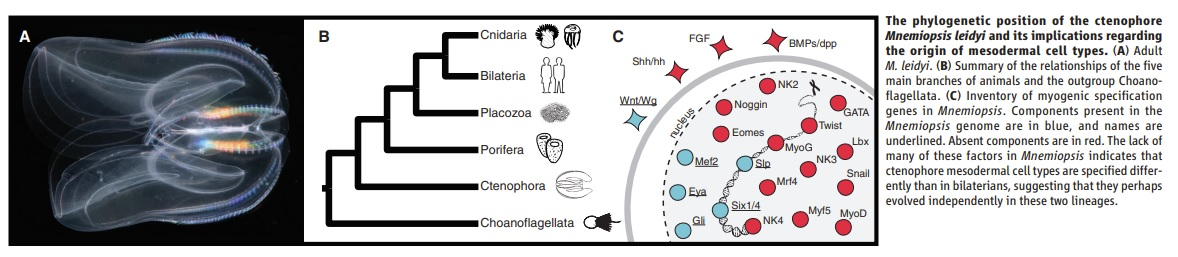
\includegraphics{https://github.com/cbarcl01/CB_BMEG591E-repository/blob/master/Group_Project/Mle.jpg}
\caption{Schema of phylogenetic position of Mnemiopsis leidyi}
\end{figure}

\hypertarget{original-study}{%
\subsubsection{1.2 Original Study}\label{original-study}}

\textless\textless\textless\textless\textless\textless\textless{} HEAD
The paper describes the first attempt to provide a reference genome to
the ctenophore \emph{Mnemiopsis leidyi}. Their results helped to propose
Ctenophores as the sister-group to all other animals, also revealing a
surprisingly complex set of neural genes similar to Sponges, providing
another interesting question: if Ctenophores are the sister group and
therefore, branching earlier than sponges, what happened to the nervous
system in sponges? The results were provoking as they shook established
hypothesis for the earliest branches of the animal tree of life. With
the goal of understanding the emergence of multicellularity in animals,
it only makes sense to spend efforts into having a reliable reference
genome to one of the most promising model organisms for this research
question {[}10{]}.

\hypertarget{sample-collection-and-genome-assembly}{%
\subparagraph{1.2.1 Sample collection and Genome
Assembly}\label{sample-collection-and-genome-assembly}}

Ryan et al collected two wild animals from the Vineyard Sound near Woods
Hole, Massachussets (Fig. 2) {[}10{]}. Those animals were
self-fertilized and DNA was isolated from the resulting embryos of one
of them. Details of the DNA isolation protocol were not disclosed, but
the authors mention the use of ``GS FLX Titanium Rapid Library
Preparation Kit'' and the ``GS FLX Titanium Library Paired End Adaptors
Kit''. The resulting isolated DNA was used for sequencing using a Roche
454 Genome Sequencer FLX machine located at the Roche Applied Science
centre in Indianapolis, IN. 7,334,972 raw reads with an Average read
length of 339 bases were generated in nine runs, yielding 2.5 Gb of
sequence.

\begin{figure}
\centering
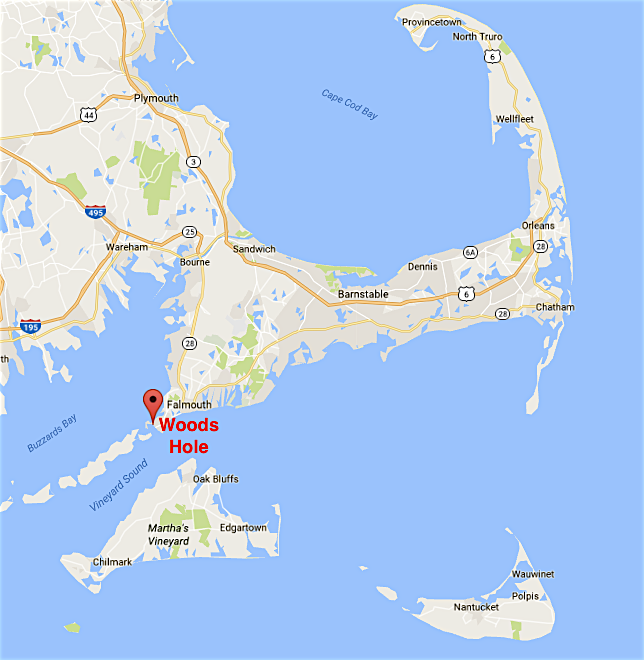
\includegraphics{https://github.com/cbarcl01/CB_BMEG591E-repository/blob/master/Group_Project/woodshole.png}
\caption{Location where wild ctenophores were collected.}
\end{figure}

Raw reads were then submitted for assembly using the Phusion assembler
{[}14{]}, resulting in 24,884 contigs with a total of 150,340,428 bases
and a reported N50 of 11,936 bases. The authors proceeded to sequence
the embryos of the second wild animal using Illumina GA-iiX system. The
resulting paired-end reads were filtered, mapped to the 24,884 assembled
contigs using Illumina's short read aligner ELAND, and integrated into
Phusion's scaffolding step. This resulted in 5,100 scaffolds with an N50
of 187 Kb and an coverage of 160X.

\hypertarget{evaluation-of-completeness-and-correctness-of-genome-assembly}{%
\paragraph{1.2.2 Evaluation of completeness and correctness of genome
assembly}\label{evaluation-of-completeness-and-correctness-of-genome-assembly}}

\hypertarget{the-authors-extracted-15752-m.-leidyi-expressed-sequence-tags-ests-and-aligned-them-to-their-assembled-genome-using-blat-15-v.-34x12-with-default-parameters.-they-evaluated-their-alignment-using-a-software-developed-by-their-group-called-baa.pl-16-later-reformed-into-isoblat-httpsgithub.comjosephryanisoblatblobmastermakefile.pl-and-obtained}{%
\section{\texorpdfstring{The authors extracted 15,752 M. leidyi
Expressed Sequence Tags (ESTs) and aligned them to their assembled
genome using BLAT {[}15{]} v. 34x12 with default parameters. They
evaluated their alignment using a software developed by their group
called baa.pl {[}16{]} later reformed into Isoblat
(\url{https://github.com/josephryan/isoblat/blob/master/Makefile.PL})
and
obtained:}{The authors extracted 15,752 M. leidyi Expressed Sequence Tags (ESTs) and aligned them to their assembled genome using BLAT {[}15{]} v. 34x12 with default parameters. They evaluated their alignment using a software developed by their group called baa.pl {[}16{]} later reformed into Isoblat (https://github.com/josephryan/isoblat/blob/master/Makefile.PL) and obtained:}}\label{the-authors-extracted-15752-m.-leidyi-expressed-sequence-tags-ests-and-aligned-them-to-their-assembled-genome-using-blat-15-v.-34x12-with-default-parameters.-they-evaluated-their-alignment-using-a-software-developed-by-their-group-called-baa.pl-16-later-reformed-into-isoblat-httpsgithub.comjosephryanisoblatblobmastermakefile.pl-and-obtained}}

The paper describes the first attempt to provide a reference genome to
the ctenophore \emph{Mnemiopsis leidyi}. Their results helped to propose
Ctenophores as the sister-group to all other animals, also revealing a
surprisingly complex set of neural genes similar to Sponges, providing
another interesting question: if Ctenophores are the sister group and
therefore, branching earlier than sponges, what happened to the nervous
system in sponges? The results were provoking as they shook established
hypothesis for the earliest branches of the animal tree of life. With
the goal of understanding the emergence of multicellularity in animals,
it only makes sense to spend efforts into having a relaible reference
genome to one of the most promising model organisms for this research
question.

\hypertarget{sample-collection-and-genome-assembly-1}{%
\subparagraph{1.2.1 Sample collection and Genome
Assembly}\label{sample-collection-and-genome-assembly-1}}

Ryan et al collected two wild animals from the Vineyard Sound near Woods
Hole, Massachussets (Fig. 2) {[}Ryan paper ref{]}. The animals were
self-fertilized and DNA was isolated from one of the resulting embryos.
Full details of the DNA isolation protocol were not disclosed, although
the use of ``GS FLX Titanium Rapid Library Preparation Kit'' and ``GS
FLX Titanium Library Paired End Adaptors Kit'' were mentioned. The
resulting isolated DNA was used for sequencing using a Roche 454 Genome
Sequencer FLX machine located at the Roche Applied Science centre in
Indianapolis, IN. In total, 7,334,972 raw reads with an Average read
length of 339 bases were generated in nine runs, yielding 2.5 Gb of
sequence.

\begin{figure}
\centering
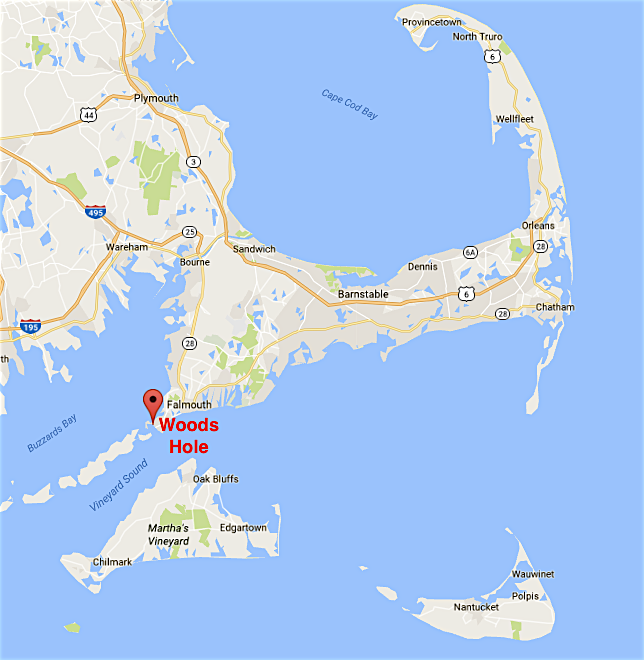
\includegraphics{https://github.com/cbarcl01/CB_BMEG591E-repository/blob/master/Group_Project/woodshole.png}
\caption{Location where wild ctenophores were collected.}
\end{figure}

Raw reads were submitted for assembly using the Phusion assembler
{[}phusion reference{]}, resulting in 24,884 contigs with a total of
150,340,428 bases and a reported N50 of 11,936 bases. The authors
proceeded to sequence the embryos of the second wild animal using
Illumina GA-iiX system. The resulting paired-end reads were filtered,
mapped to the 24,884 assembled contigs using Illumina's short read
aligner ELAND, and integrated into Phusion's scaffolding step. This
resulted in 5,100 scaffolds with an N50 of 187 Kb and an coverage of
160X.

\hypertarget{evaluation-of-completeness-and-correctness-of-genome-assembly-1}{%
\paragraph{1.2.2 Evaluation of completeness and correctness of genome
assembly}\label{evaluation-of-completeness-and-correctness-of-genome-assembly-1}}

In the original study 15,752 M. leidyi Expressed Sequence Tags (ESTs)
were downloaded from GenBank and aligned to the assembled genome using
BLAT {[}Blat ref{]} v. 34x12 with default parameters. The alignment was
assessed using a software developed by the authors called baa.pl
{[}baa.pl ref{]} later reformed into Isoblat {[}github link to
Isoblat{]}. The results were as follows:
\textgreater\textgreater\textgreater\textgreater\textgreater\textgreater\textgreater{}
654e06a9d4342becd5ba14dbf3e52919507519c6

\begin{enumerate}
\def\labelenumi{\arabic{enumi})}
\tightlist
\item
  99.4\% of the transcripts were mapped with BLAT
\item
  98.2\% of the positions in the mapped transcripts were aligned
\item
  95.2\% of the transcripts mapped to a single scaffold.
\end{enumerate}

They further extracted and sequenced 79 Mb paired-end/83 Mb single-end
RNA reads from \emph{M. leidyi} embryos through Illumina GA-II platform
and assembled them using Trinity {[}17{]}. Their final assembly had
32,630 for paired-end and 27,315 for single-end transcripts
respectively. They proceeded to align their Trinity-assembled
transcripts to BLAT and analyze it through baa.pl with default
parameters and generated the following statistics:

\begin{enumerate}
\def\labelenumi{\arabic{enumi})}
\tightlist
\item
  99.2\% of the transcripts were mapped with BLAT
\item
  98.1\% of the positions in the mapped transcripts were aligned
\item
  92.7\% of the transcripts mapped to a single scaffold.
\end{enumerate}

Thus, they conclude that their assembly is likely complete and correctly
assembled. Further repeat analysis indicates allowed them to estimate a
genome size of 150 Mb, which configures this genome to be one of the
smallest 7\% known genomes {[}10{]}.

\hypertarget{gene-prediction-pipeline}{%
\paragraph{1.2.3 Gene Prediction
pipeline}\label{gene-prediction-pipeline}}

The authors provided a complex, in-depth pipeline for gene prediction
with no common pattern between automated and manual steps. Firstly, the
authors sequenced another round of RNA-seq data, resulting in 162 Mb of
RNA-seq data originating from mixed stage embryos (ranging from a few
hours up until 15 hours post-fertilization). These reads were mapped to
their assembled genome using TopHat {[}18{]} and then assembled into
49,850 transcript fragments using Cufflinks {[}19{]}.

\textless\textless\textless\textless\textless\textless\textless{} HEAD
They then loaded the 49,850 Cufflink fragments, the 15,752 publicly
available ESTs, and additional 161 alleged publicly available cDNA
sequences into PASA {[}20{]} without providing details of this step.
They masked the genome with a repeat library, excluding from the masking
regions where RNA-seq mappings overlapped, resulting in 53,244 regions
and 7,387,140 base pairs of sequence. This data was then submitted to
several prediction softwares: FGENESH {[}21{]}; AUGUSTUS {[}22{]}
(version\_2.3.1); HMMgene {[}23{]} (version\_1.1); and GenomeScan
{[}24{]} (version\_0.1). They evaluated the predicted models using
Evidence Modeler (EVM version\_r03062010) {[}25{]}. In total, the
authors established that the genome contains 16,548 predicted genes (or
protein-coding loci), making up 58\% of its total length, with 44\% of
those loci being homologous to known genes in non-ctenophores.\\
======= Next, the 49,850 Cufflink fragments, 15,752 publicly available
ESTs, and additional 161 publicly available cDNA sequences were loaded
into PASA {[}pasa ref{]} without providing details of this step. The
genome was masked with a repeat library, excluding from masking regions
where RNA-seq mappings overlapped, resulting in 53,244 regions and
7,387,140 base pairs of sequence. Several prediction softwares were
called including: GENESH {[}genesh ref{]}; AUGUSTUS {[}augustus ref{]}
(version\_2.3.1); HMMgene {[}hmmgene ref{]} (version\_1.1); and
GenomeScan {[}genomescan ref{]} (version\_0.1 and the predicted models
were then evaluated using Evidence Modeler (EVM version\_r03062010)
{[}EVM ref{]}.

In total, the authors established that the genome contains 16,548
predicted genes (or protein-coding loci), making up 58\% of its total
length, with 44\% of those loci being homologous to known genes in
non-ctenophores.\\
\textgreater\textgreater\textgreater\textgreater\textgreater\textgreater\textgreater{}
654e06a9d4342becd5ba14dbf3e52919507519c6

\hypertarget{phylogenetic-analysis}{%
\paragraph{1.2.4 Phylogenetic analysis}\label{phylogenetic-analysis}}

The newly assembled \emph{Mnemiopsis leidyi} genome was used in
assessment of gene sequence evolution, to identify the phylogenetic
placement of Ctenophora compared to other non-bilaterian clades. A
`genome set' with whole genomes from 13 animals (19.6\% missing data)and
an EST set which included partial data 58 animals (64,9\% missing data),
was analysed using maximum likelihood and Bayesian methods. The runs
were computationally intensive, with runs taking 205 days on average for
the Bayesian analysis of the EST data without convergence. Evidence
supported a sister relationship between Cnidaria and Bilateria, however
the study highlighted the importance of further analysis as more data
becomes available.

\hypertarget{re-analysis}{%
\subsubsection{1.3 Re-analysis}\label{re-analysis}}

This study was chosen as it provides a much needed reference genome to a
model organism in studies related to the origins of multicellularity and
particularly the phylogenetic organization of the earliest-branching
Metazoans - the phylogenetic placement of Ctenophores compared to other
non-bilaterans is still widely debated. The original study was
undertaken in 2011 and published in 2013 {[}10{]}, since then, many of
the tools that the paper used have either changed or received updates,
while some are no longer maintained and more data has been made
available for gene annotation.

In our re-analysis, in the absence of raw reads we will investigate the
files to confirm the number of contigs and scaffolds before running the
following analysis to assess for completeness of the assembly:

\begin{itemize}
\tightlist
\item
  Replicate and validate the alignment of ESTs as seen in the original
  study using BLAT
\item
  Replicate and validate the alignment of transcripts as seen in the
  original study using BLAT
\item
  Compare alignment of ESTs with original tool BLAT and Bowtie2
\item
  Design Perl script to assess GC content in absence of fastqc files and
  compare the output with publicly available scripts
\end{itemize}

Following this assessment for correctness of assembly, we will undertake
part of the following analyses:

\begin{itemize}
\tightlist
\item
  Annotation
\item
  Phylogeny
\end{itemize}

\hypertarget{workflow-methods-and-results}{%
\subsection{2 Workflow: Methods and
Results}\label{workflow-methods-and-results}}

\hypertarget{data-gathering}{%
\subsubsection{2.1 Data gathering}\label{data-gathering}}

\hypertarget{mnemiopsis-genome-portal}{%
\paragraph{2.1.1 Mnemiopsis Genome
Portal}\label{mnemiopsis-genome-portal}}

The data was accessed from the Mnemiopsis Genome Portal {[}26{]}, a
public database for genomic and functional information on \emph{M.
leidyi}. The Portal is regularly maintained, with a BLAST interface as
well as a visualization tool which allows exploration of the scaffolds
and RNA seq data, similarly to the IGV Browser {[}26{]}. Alternatively
the data from this study can be obtained from GenBank
\href{https://www.ncbi.nlm.nih.gov/assembly/GCA_000226015.1}{here}. The
files from both resources are the same, scaffold and contig .fasta
files. Raw reads are not publicly available.

\textbf{LOADING GENOME}

\begin{Shaded}
\begin{Highlighting}[]

\CommentTok{\#Download the scaffolds to local machine then imported to server using pscp}

\ExtensionTok{pscp}\NormalTok{ {-}P 22 {-}r C:\textbackslash{}Users\textbackslash{}heavy\textbackslash{}Documents\textbackslash{}bmeg{-}591\textbackslash{}BMEG{-}591{-}Rep\textbackslash{}Project\textbackslash{}MlScaffold09.nt.gz gdalba@gi{-}edu{-}sv2.bme.ubc.ca:/home/gdalba/MlScaffold09.nt.gz}

\CommentTok{\#OR Download the contigs directly to server using wget {-} This comes from the alternative source, not the Genome Portal.}

\FunctionTok{wget}\NormalTok{ {-}o ./Project/AGCP01.zip https://sra{-}download.ncbi.nlm.nih.gov/traces/wgs03/wgs\_aux/AG/CP/AGCP01/AGCP01.1.fsa\_nt.gz}

\CommentTok{\#On server, unziped using gzip}

\FunctionTok{gzip}\NormalTok{ {-}d MlScaffold09.nt.gz}

\CommentTok{\#We confirmed the 5,100 scaffolds through:}

\FunctionTok{grep}\NormalTok{ {-}c }\StringTok{"\^{}\textgreater{}"}\NormalTok{ MlScaffold09.nt}
\ExtensionTok{5100}
\end{Highlighting}
\end{Shaded}

\textbf{LOADING ESTs}

The 15,752 publicly available ESTs were identified and downloaded from
\url{https://research.nhgri.nih.gov/mnemiopsis/download/download.cgi?dl=est}.
Additionally we queried GenBank to confirm no additional ESTs had been
added since the original study.

\begin{Shaded}
\begin{Highlighting}[]

\CommentTok{\#Imported to server using pscp}

\ExtensionTok{pscp}\NormalTok{ {-}P 22 {-}r C:\textbackslash{}Users\textbackslash{}heavy\textbackslash{}Documents\textbackslash{}bmeg{-}591\textbackslash{}BMEG{-}591{-}Rep\textbackslash{}Project\textbackslash{}MlESTs.gz gdalba@gi{-}edu{-}sv2.bme.ubc.ca:/home/gdalba/MlESTs.gz}

\CommentTok{\#On server, unziped using gzip}

\FunctionTok{gzip}\NormalTok{ {-}d MlESTs.gz}

\CommentTok{\#We confirmed the 15,752 ESTs through:}
\FunctionTok{grep}\NormalTok{ {-}c }\StringTok{"\^{}\textgreater{}"}\NormalTok{ MlESTs.fa}
\ExtensionTok{15752}
\end{Highlighting}
\end{Shaded}

\textbf{LOADING RNA DATA}

35,203 assembled transcripts using Trinity were downloaded from
\url{https://research.nhgri.nih.gov/mnemiopsis/download/download.cgi?dl=transcript}
and loaded into the server.

\begin{Shaded}
\begin{Highlighting}[]

\CommentTok{\#Imported to server using pscp}

\ExtensionTok{pscp}\NormalTok{ {-}P 22 {-}r C:\textbackslash{}Users\textbackslash{}heavy\textbackslash{}Documents\textbackslash{}bmeg{-}591\textbackslash{}BMEG{-}591{-}Rep\textbackslash{}Project\textbackslash{}Ml\_Trinity\_transcripts.fa.gz gdalba@gi{-}edu{-}sv2.bme.ubc.ca:/home/gdalba/Ml\_Trinity\_transcripts.fa.gz}

\CommentTok{\#On server, unziped using gzip}

\FunctionTok{gzip}\NormalTok{ {-}d Ml\_Trinity\_transcripts.fa.gz}

\CommentTok{\#We confirmed the 15,752 ESTs through:}
\FunctionTok{grep}\NormalTok{ {-}c }\StringTok{"\^{}\textgreater{}"}\NormalTok{ Ml\_Trinity\_transcripts.fa}
\ExtensionTok{35203}
\end{Highlighting}
\end{Shaded}

\hypertarget{evaluation-of-correctness}{%
\subsubsection{2.2 Evaluation of
Correctness}\label{evaluation-of-correctness}}

\hypertarget{bowtie-x-blat}{%
\paragraph{2.2.1 Bowtie x BLAT}\label{bowtie-x-blat}}

\textbf{BLAT}

\textbf{BLAT INSTALLATION}

BLAT v. 36x2 was installed through our conda environment:

\begin{Shaded}
\begin{Highlighting}[]

\ExtensionTok{conda}\NormalTok{ activate gdalba{-}conda}

\ExtensionTok{conda}\NormalTok{ install ucsc{-}blat}
\end{Highlighting}
\end{Shaded}

\textbf{RUNNING BLAT}

We ran BLAT with default parameters as described in the paper as
follows:

\begin{Shaded}
\begin{Highlighting}[]

\ExtensionTok{blat}\NormalTok{ MlScaffold09.nt MlESTs mle\_blatalign.psl}

\ExtensionTok{Loaded}\NormalTok{ 155865547 letters in 5100 sequences}
\ExtensionTok{Searched}\NormalTok{ 10552828 bases in 15752 sequences}
\ExtensionTok{mle\_blatalign.psl}
\end{Highlighting}
\end{Shaded}

\textbf{BAA.PL/ISOBLAT INSTALLATION}

baa.pl/Isoblat is a tool that uses transcripts to assess assembly
quality. Using transcripts X assembled genome BLAT output as its input,
it yields the following statistics (as seen earlier): Total \% mapped,
average \% coverage of a mapping, and number of transcripts mapping to a
single contig/scaffold.

We cloned baa.pl/Isoblat github repo
(\url{https://github.com/josephryan/isoblat}) on our own machines and
imported it to our server:

\begin{Shaded}
\begin{Highlighting}[]

\CommentTok{\#Importing baa.pl/Isoblat to server}

\ExtensionTok{pscp}\NormalTok{ {-}P 22 {-}r C:\textbackslash{}Users\textbackslash{}heavy\textbackslash{}Documents\textbackslash{}bmeg{-}591\textbackslash{}BMEG{-}591{-}Rep\textbackslash{}Project\textbackslash{}baa.pl\textbackslash{}isoblat gdalba@gi{-}edu{-}sv2.bme.ubc.ca:/home/gdalba/baa.pl}

\CommentTok{\#Installing baa.pl/Isoblat}

\FunctionTok{perl}\NormalTok{ Makefile.PL}
\FunctionTok{make}
\FunctionTok{make}\NormalTok{ install}
\end{Highlighting}
\end{Shaded}

\textbf{RUNNING BAA.PL/ISOBLAT}

We ran baa.pl/Isoblat with default parameters as described in the paper
as follows:

\begin{Shaded}
\begin{Highlighting}[]

\ExtensionTok{isoblat}\NormalTok{ {-}{-}max\_gap\_to\_consider\_missing=5 {-}{-}min\_to\_count\_as\_coverage=5 mle\_blatalign.psl MlESTs.fa }\OperatorTok{2\textgreater{}}\NormalTok{/dev/null}

\CommentTok{\# running version 0.31 of isoblat}
\CommentTok{\# run with this command: /home/gdalba/.conda/envs/gdalba{-}conda/bin/isoblat mle\_blatalign.psl MlESTs.fa}
\CommentTok{\# $max\_gap\_to\_consider\_missing = 5}
\CommentTok{\# $min\_to\_count\_as\_coverage    = 5}

\ExtensionTok{Ratio}\NormalTok{ of transcripts with a BLAT entry (15665/15752)}\BuiltInTok{:}\NormalTok{ 0.99447689182326}
\end{Highlighting}
\end{Shaded}

As it can be seen, only one of the three expected statistics were
yielded as output. We are unsure of the reasons why baa.pl/Isoblat
algorithm fails to capture enough information for the other two
calculations (\% of transcripts positions successfully aligned and \% of
transcripts that mapped to a single scaffold). We attempted to
troubleshoot the algorithm itself to no luck. The algorithm attempted to
read non-existent lines, returning non-numeric values and divisions
either by non-numeric values or by zero.

\textbf{RUNNING BLAT + BAA.PL/ISOBLAT FOR RNA DATA}

We repeated the above steps using Trinity-assembled transcripts:

\begin{Shaded}
\begin{Highlighting}[]

\ExtensionTok{blat}\NormalTok{ MlScaffold09.fa Ml\_Trinity\_transcripts.fa blatrnaalign.psl}
\ExtensionTok{Loaded}\NormalTok{ 155865547 letters in 5100 sequences}
\ExtensionTok{Searched}\NormalTok{ 29298205 bases in 35203 sequences}

\ExtensionTok{isoblat}\NormalTok{ /home/gdalba/blatrnaalign.psl /home/gdalba/Ml\_Trinity\_transcripts.fa}
\CommentTok{\# running version 0.31 of isoblat}
\CommentTok{\# run with this command: /home/gdalba/.conda/envs/gdalba{-}conda/bin/isoblat /home/gdalba/blatrnaalign.psl /home/gdalba/Ml\_Trinity\_transcripts.fa}
\CommentTok{\# $max\_gap\_to\_consider\_missing = 5}
\CommentTok{\# $min\_to\_count\_as\_coverage    = 5}
\ExtensionTok{Ratio}\NormalTok{ of transcripts with a BLAT entry (34815/35203)}\BuiltInTok{:}\NormalTok{ 0.988978212084197}
\end{Highlighting}
\end{Shaded}

\textbf{BOWTIE2}

We also attempted the same correctness evaluation using a different
aligner - Bowtie2 {[}27{]}. We performed steps similarly as to what was
described in class. The main goal was to comparte different alignment
tools and their output. Bowtie2 was already installed server-side.

\textbf{CREATING AN INDEX}

\begin{Shaded}
\begin{Highlighting}[]
\ExtensionTok{bowtie2{-}build}\NormalTok{ MlScaffold09.nt /home/gdalba/genome\_index/Mlindex}
\end{Highlighting}
\end{Shaded}

\textbf{RUNNING BOWTIE2 WITH ESTs}

\begin{Shaded}
\begin{Highlighting}[]
\ExtensionTok{bowtie2}\NormalTok{ {-}x /home/gdalba/genome\_index/Mlindex {-}f MlESTs {-}S /home/gdalba/mle\_align.index}

\ExtensionTok{15752}\NormalTok{ reads}\KeywordTok{;} \ExtensionTok{of}\NormalTok{ these:}
  \ExtensionTok{15752}\NormalTok{ (100.00\%) }\ExtensionTok{were}\NormalTok{ unpaired}\KeywordTok{;} \ExtensionTok{of}\NormalTok{ these:}
    \ExtensionTok{6989}\NormalTok{ (44.37\%) }\ExtensionTok{aligned}\NormalTok{ 0 times}
    \ExtensionTok{8562}\NormalTok{ (54.36\%) }\ExtensionTok{aligned}\NormalTok{ exactly 1 time}
    \ExtensionTok{201}\NormalTok{ (1.28\%) }\ExtensionTok{aligned} \OperatorTok{\textgreater{}}\NormalTok{1 times}
\ExtensionTok{55.63\%}\NormalTok{ overall alignment rate}
\end{Highlighting}
\end{Shaded}

\textbf{RUNNING BOWTIE2 WITH TRINITY-ASSEMBLED RNA TRANSCRIPTS}

\begin{Shaded}
\begin{Highlighting}[]
\ExtensionTok{bowtie2}\NormalTok{ {-}x /home/gdalba/genome\_index/Mlindex {-}f Ml\_Trinity\_transcripts.fa {-}S /home/gdalba/mle\_rnaalign.index}


\ExtensionTok{35203}\NormalTok{ reads}\KeywordTok{;} \ExtensionTok{of}\NormalTok{ these:}
  \ExtensionTok{35203}\NormalTok{ (100.00\%) }\ExtensionTok{were}\NormalTok{ unpaired}\KeywordTok{;} \ExtensionTok{of}\NormalTok{ these:}
    \ExtensionTok{16346}\NormalTok{ (46.43\%) }\ExtensionTok{aligned}\NormalTok{ 0 times}
    \ExtensionTok{17177}\NormalTok{ (48.79\%) }\ExtensionTok{aligned}\NormalTok{ exactly 1 time}
    \ExtensionTok{1680}\NormalTok{ (4.77\%) }\ExtensionTok{aligned} \OperatorTok{\textgreater{}}\NormalTok{1 times}
\ExtensionTok{53.57\%}\NormalTok{ overall alignment rate}
\end{Highlighting}
\end{Shaded}

\hypertarget{assessing-gc-content}{%
\subsubsection{2.3 Assessing GC Content}\label{assessing-gc-content}}

We employed 2 distinct GC content measurement approaches: a manual
approach and a pre-built script.

\textbf{BIOBASH SCRIPTS}

We cloned the Github repo (\url{https://github.com/gibbslab/biobash})
containing several general utilities Bioinformatics scripts called
BIOBASH, developed in Bash language. We imported the scripts using pscp
and converted scripts of interest using the command ``dos2unix -k -o '':

\textbf{BIOBASH INSTALLATION}

\begin{Shaded}
\begin{Highlighting}[]

\ExtensionTok{{-}P}\NormalTok{ 22 {-}r C:\textbackslash{}Users\textbackslash{}heavy\textbackslash{}Documents\textbackslash{}bmeg{-}591\textbackslash{}BMEG{-}591{-}Rep\textbackslash{}Project\textbackslash{}biobash gdalba@gi{-}edu{-}sv2.bme.ubc.ca:/home/gdalba/scripts}

\ExtensionTok{dos2unix}\NormalTok{ {-}k {-}o installbiobash}
\FunctionTok{chmod}\NormalTok{ +x installbiobash}
\ExtensionTok{./installbiobash}
\end{Highlighting}
\end{Shaded}

To test if the BIOBASH set os scripts were working, we repeated the
validation of assembly file MlScaffold09.nt (converted into fasta) with
bb\_count\_seqs script (script that count sequences) after
troubleshooting and fixing minimal problems within the script:

\begin{Shaded}
\begin{Highlighting}[]

\ExtensionTok{dos2unix}\NormalTok{ {-}k {-}o bb\_count\_seqs}
\FunctionTok{chmod}\NormalTok{ +x bb\_count\_seqs}
\ExtensionTok{./bb\_count\_seqs}\NormalTok{ /home/gdalba/MlScaffold09.fa}
\ExtensionTok{5100}\NormalTok{ Scaffolds}
\end{Highlighting}
\end{Shaded}

We then ran bb\_get\_GC\_content after troubleshooting and fixing
minimal problems within the script, which required a .fa file with a
single header:

\begin{Shaded}
\begin{Highlighting}[]

\FunctionTok{grep}\NormalTok{ {-}v }\StringTok{"\textgreater{}"}\NormalTok{ MlScaffold09.fa}\OperatorTok{\textgreater{}} \OperatorTok{\textgreater{}}\NormalTok{ MlScaffold09\_singleseq.fa}
\end{Highlighting}
\end{Shaded}

\begin{Shaded}
\begin{Highlighting}[]

\ExtensionTok{dos2unix}\NormalTok{ {-}k {-}o bb\_get\_GC\_content}
\FunctionTok{chmod}\NormalTok{ +x bb\_get\_GC\_content}
\ExtensionTok{./bb\_get\_GC\_content}\NormalTok{ /home/gdalba/MlScaffold09\_singleseq.fa}
\ExtensionTok{37}
\end{Highlighting}
\end{Shaded}

bb\_get\_GC\_content reported a GC content of 37\%. We then applied two
perl approaches

\textbf{PERL: GC CONTENT}

\begin{Shaded}
\begin{Highlighting}[]

\FunctionTok{perl}\NormalTok{ {-}lane }\StringTok{\textquotesingle{}unless (/\^{}\textgreater{}/) \{ $l += length(); $gc++ while /[GC]/ig \} END \{ print $gc/$l\}\textquotesingle{}}\NormalTok{ /home/gdalba/MlScaffold09.fa}
\ExtensionTok{0.374857844626818}
\end{Highlighting}
\end{Shaded}

\textbf{PERL: GC CONTENT PER SCAFFOLD}

\begin{Shaded}
\begin{Highlighting}[]

\FunctionTok{perl}\NormalTok{ {-}lane }\StringTok{\textquotesingle{}if (/\^{}\textgreater{}(.+)/) \{}
\StringTok{ printf "\%s \%d \%.2f\textbackslash{}n", $n, $l, $gc/$l if $l;}
\StringTok{ $n = $1; $l = 0; $gc = 0;}
\StringTok{\} else \{}
\StringTok{ $l += length($\_);}
\StringTok{ $gc++ while /[GC]/ig;}
\StringTok{\} END \{}
\StringTok{ printf "\%s \%d \%.2f\textbackslash{}n", $n, $l, $gc/$l if $l;}
\StringTok{\}\textquotesingle{}}\NormalTok{ /home/gdalba/MlScaffold09.fa}

\ExtensionTok{Resulting}\NormalTok{ Average: 0,3754960784}
\end{Highlighting}
\end{Shaded}

\hypertarget{annotation}{%
\subsubsection{2.4 Annotation}\label{annotation}}

We installed Augustus and its dependencies through conda:

\begin{Shaded}
\begin{Highlighting}[]

\ExtensionTok{conda}\NormalTok{ install {-}c bioconda augustus}
\ExtensionTok{conda}\NormalTok{ install {-}c anaconda libboost}
\end{Highlighting}
\end{Shaded}

We prepared a hints file using the ESTs aligned to the genome (through
the BLAT output) with aid of the following tutorial:
\url{https://vcru.wisc.edu/simonlab/bioinformatics/programs/augustus/docs/tutorial2015/prediction.html}.
Originally, the authors loaded the \emph{M. leidyi} RNA-seq reads
(49,850 Cufflinks transcripts), publicly available mRNAs (161) and
publicly available ESTs (15,752). We loaded the Cufflink Transcripts and
the publicly available ESTs through the following:

\begin{Shaded}
\begin{Highlighting}[]

\CommentTok{\#Ran filterPSL to exclude alignments below 80\% of query length coverage}

\CommentTok{\#mle\_blatalign.psl = BLAT alignment of ESTs to the assembled genome.}
\CommentTok{\#blatrnaalgin.psl = Trinity assembled transcripts}
\CommentTok{\#mle\_cuffalign.psl = Cufflinks assembled transcripts}

\FunctionTok{cat}\NormalTok{ mle\_blatalign.psl }\KeywordTok{|} \FunctionTok{perl}\NormalTok{ /home/gdalba/.conda/pkgs/augustus{-}3.2.2{-}0/scripts/filterPSL.pl {-}{-}best {-}{-}minCover=80 }\OperatorTok{\textgreater{}}\NormalTok{ filterMle\_blatalign.psl}

\FunctionTok{cat}\NormalTok{ blatrnaalign.psl }\KeywordTok{|} \FunctionTok{perl}\NormalTok{ /home/gdalba/.conda/pkgs/augustus{-}3.2.2{-}0/scripts/filterPSL.pl {-}{-}best {-}{-}minCover=80 }\OperatorTok{\textgreater{}}\NormalTok{ filterMle\_rnaalign.psl}

\FunctionTok{cat}\NormalTok{ mle\_cuffalign.psl }\KeywordTok{|} \FunctionTok{perl}\NormalTok{ /home/gdalba/.conda/pkgs/augustus{-}3.2.2{-}0/scripts/filterPSL.pl {-}{-}best {-}{-}minCover=80 }\OperatorTok{\textgreater{}}\NormalTok{ filterMle\_cuffalign.psl}

\CommentTok{\#As we can see, this filtering step reduced the amount of relevant alignments from 165481 to 14505, 318457 to 31271, and 2440089 to 50107 for mle\_blatalign.psl, blatrnaalign.psl, and mle\_cuffalign.psl respectively.}

\FunctionTok{wc}\NormalTok{ {-}l mle\_blatalign.psl filterMle\_blatalign.psl}
  \ExtensionTok{165481}\NormalTok{ mle\_blatalign.psl}
   \ExtensionTok{14505}\NormalTok{ filterMle\_blatalign.psl}
  \ExtensionTok{179986}\NormalTok{ total}
  
\FunctionTok{wc}\NormalTok{ {-}l blatrnaalign.psl filterMle\_rnaalign.psl}
  \ExtensionTok{318457}\NormalTok{ blatrnaalign.psl}
   \ExtensionTok{31271}\NormalTok{ filterMle\_rnaalign.psl}
  \ExtensionTok{349728}\NormalTok{ total}

\FunctionTok{wc}\NormalTok{ {-}l mle\_cuffalign.psl filterMle\_cuffalign.psl}
  \ExtensionTok{2440089}\NormalTok{ mle\_cuffalign.psl}
    \ExtensionTok{50107}\NormalTok{ filterMle\_cuffalign.psl}
  \ExtensionTok{2490196}\NormalTok{ total}

\CommentTok{\#We then merge the two filtered files.}

\FunctionTok{cat}\NormalTok{ filterMle\_blatalign.psl filterMle\_cuffalign.psl }\OperatorTok{\textgreater{}}\NormalTok{ combined\_cuffhints.psl}

\CommentTok{\#And run blat2hints}

\ExtensionTok{blat2hints.pl}\NormalTok{ {-}{-}nomult {-}{-}in=combined\_cuffhints.psl {-}{-}out=hints.mle.gff}
\end{Highlighting}
\end{Shaded}

With the hints file ready, we can run Augustus. Augustus was originally
trained using \emph{Amphimedon queenslandica}, a data set that is
already available through the tool itself.

\begin{Shaded}
\begin{Highlighting}[]

\ExtensionTok{augustus}\NormalTok{ {-}{-}progress=true {-}{-}species=amphimedon {-}{-}extrinsicCfgFile=extrinsic.ME.cfg {-}{-}hintsfile=hints.mle.gff MlScaffold09.fa }\OperatorTok{\textgreater{}}\NormalTok{ augustus\_annotation.gff}

\ExtensionTok{where}\NormalTok{,}
\ExtensionTok{{-}{-}progress}\NormalTok{=true shows the performance of every step}

\ExtensionTok{{-}{-}species}\NormalTok{=amphimedon indicates the training dataset, alternatively, you would train your own dataset.}

\ExtensionTok{{-}{-}extrinsicCfgFile}\NormalTok{=extrinsic.ME.cfg loads a .cfg file containing metadatafrom the hints file, for instance, and parameters that help to assess the quality of the gene prediction and accurately decide where which gene elements are in a predicted sequence. The .ME.cfg file takes into account information coming from the ESTs located within the Hints file, which is useful in our case.}

\ExtensionTok{{-}{-}hintsfile}\NormalTok{=hints.mle.gff specifies the hints we generated in the previous steps.}

\ExtensionTok{By}\NormalTok{ default, Augustus predicts on both forward and reverse.}
\end{Highlighting}
\end{Shaded}

\begin{Shaded}
\begin{Highlighting}[]

\CommentTok{\#Assessing number of predicted genes by Augustus}

\FunctionTok{awk} \StringTok{\textquotesingle{}$3=="gene"\textquotesingle{}}\NormalTok{ augustus\_annotation.gff }\KeywordTok{|} \FunctionTok{wc}\NormalTok{ {-}l}
\ExtensionTok{33354}

\ExtensionTok{Example}\NormalTok{ of Augustus output:}

\ExtensionTok{ML5014}\NormalTok{  AUGUSTUS        gene    20      829     0.87    +       .       g11104}
\ExtensionTok{ML5014}\NormalTok{  AUGUSTUS        transcript      20      829     0.87    +       .       g11104.t1}
\ExtensionTok{ML5014}\NormalTok{  AUGUSTUS        start\_codon     20      22      .       +       0       transcript\_id }\StringTok{"g11104.t1"}\KeywordTok{;} \ExtensionTok{gene\_id} \StringTok{"g11104"}\KeywordTok{;}
\ExtensionTok{ML5014}\NormalTok{  AUGUSTUS        CDS     20      829     0.87    +       0       transcript\_id }\StringTok{"g11104.t1"}\KeywordTok{;} \ExtensionTok{gene\_id} \StringTok{"g11104"}\KeywordTok{;}
\ExtensionTok{ML5014}\NormalTok{  AUGUSTUS        stop\_codon      827     829     .       +       0       transcript\_id }\StringTok{"g11104.t1"}\KeywordTok{;} \ExtensionTok{gene\_id} \StringTok{"g11104"}\KeywordTok{;}
\CommentTok{\# protein sequence = [MLQDSRSYAGTLAYSDHRLVVTRVNFKNICLCYKRHTQSSFKFDTSELTSNPTIQVKYRHSLNENLSNAVPALDPNSD}
\CommentTok{\# LNSLLESIKDAAKSSIGVTRHRKRNRSDNDEVKSLSNQRHMLRQQLNNNQSMDRTLLRSSINRLTNQIQQRLSILRSAAADAICNTISTTTDSKKMFE}

\ExtensionTok{We}\NormalTok{ can run this prediction against Mnemiopsis protein models using BLASTp (https://research.nhgri.nih.gov/mnemiopsis/sequenceserver/\#), }\ExtensionTok{the}\NormalTok{ best match (for this protein, is the protein model ML050010a, with an e{-}score of 6e{-}122) }\ExtensionTok{can}\NormalTok{ then undergo regular Blastp analysis, revealing 83\% identity (e{-}value: 4e{-}43) }\ExtensionTok{with}\NormalTok{ an uncharacterized protein found in *Octopus sinensis*.}
\end{Highlighting}
\end{Shaded}

Multiple attempts to run PASA, HMMGene, and GENESH were made, but due to
time constrains and technical challenges, we decided to run Augustus
alone. Augustus predicted 33,354 protein-coding loci. We then used
BED-tools getfasta function to extract sequences:

\begin{Shaded}
\begin{Highlighting}[]
\CommentTok{\#filters every possible sequence type into a .bed file}

\FunctionTok{awk} \StringTok{\textquotesingle{}($3=="CDS" || $3=="gene" || $3=="tRNA" || $3=="tmRNA" || $3=="ncRNA" || $3=="rRNA") \{OFS="\textbackslash{}t"; print $1,$4{-}1,$5\}\textquotesingle{}}\NormalTok{ augustus\_annotation.gff }\OperatorTok{\textgreater{}}\NormalTok{ mlegenes.bed}

\CommentTok{\#getfasta function correlates predicted sequences in .bed file back to the assembled genome and store them on a .ffn file}

\ExtensionTok{bedtools}\NormalTok{ getfasta {-}fi MlScaffold09.fa {-}bed mlegenes.bed {-}fo mle.ffn}
\end{Highlighting}
\end{Shaded}

When mapping back to the genome, we obtain 29,875 genes. This file can
then be used to manually curate sequences following the previously
mentioned BLASTp approach.

\hypertarget{phylogeny}{%
\subsubsection{2.4 Phylogeny}\label{phylogeny}}

\begin{quote}
\begin{quote}
\begin{quote}
\begin{quote}
\begin{quote}
\begin{quote}
\begin{quote}
654e06a9d4342becd5ba14dbf3e52919507519c6
\end{quote}
\end{quote}
\end{quote}
\end{quote}
\end{quote}
\end{quote}
\end{quote}

In the original study, phylogenetic analysis was conducted using
PhyloBayes ``a Bayesian Monte Carlo Markov Chain (MCMC) sampler for
phylogenetic reconstruction'', comparing the whole genomes of 13
different animals in the `Genome set' vs the EST data available in
GenBank from 58 different animals in the `EST set' {[}10{]}.
Unfortunately, one of the runs for EST alone took 204 days and as such
was not reproducible for this assignment.

Phylogenetic analysis allows researchers the opportunity to identify
potential similarity between species, indicating lineage and in the case
of Ctenophora hopefully offer further insights into their placement as
the most basal animal lineage {[}10, 11{]}. In conjunction with
annotation, phylogeny could be used to assess orthologs and genetically
conserved regions that can be traced back to the root of metazoan
divergence. Consequently, instead of replicating the whole genome or EST
phylogenetics (due to the aforementioned time limitations), we have
compared a significant gene region of interest to scientists in the
origins of animal multicellularity.

In the original study, Ryan et al.~suggested through phylogenetic
analysis that ionotropic glutamate receptors from \emph{M. leidyi} form
a sister clade to the bilaterian glutamate receptors. The gene region of
interest was identified as ML00441a and both the transcript sequence and
predicted protein sequence can be viewed
\href{https://research.nhgri.nih.gov/mnemiopsis/wiki/index.php/ML00441a}{here}.

\hypertarget{mnemiopsis-genome-project-portal-track-viewer}{%
\paragraph{2.4.1 Mnemiopsis Genome Project Portal: Track
Viewer}\label{mnemiopsis-genome-project-portal-track-viewer}}

The following is a snap shot from the Mnemiopsis leidyi genome portal
track for the gene region of interest. This viewer can be interrogated
similarly to the IGV.

\begin{figure}
\centering
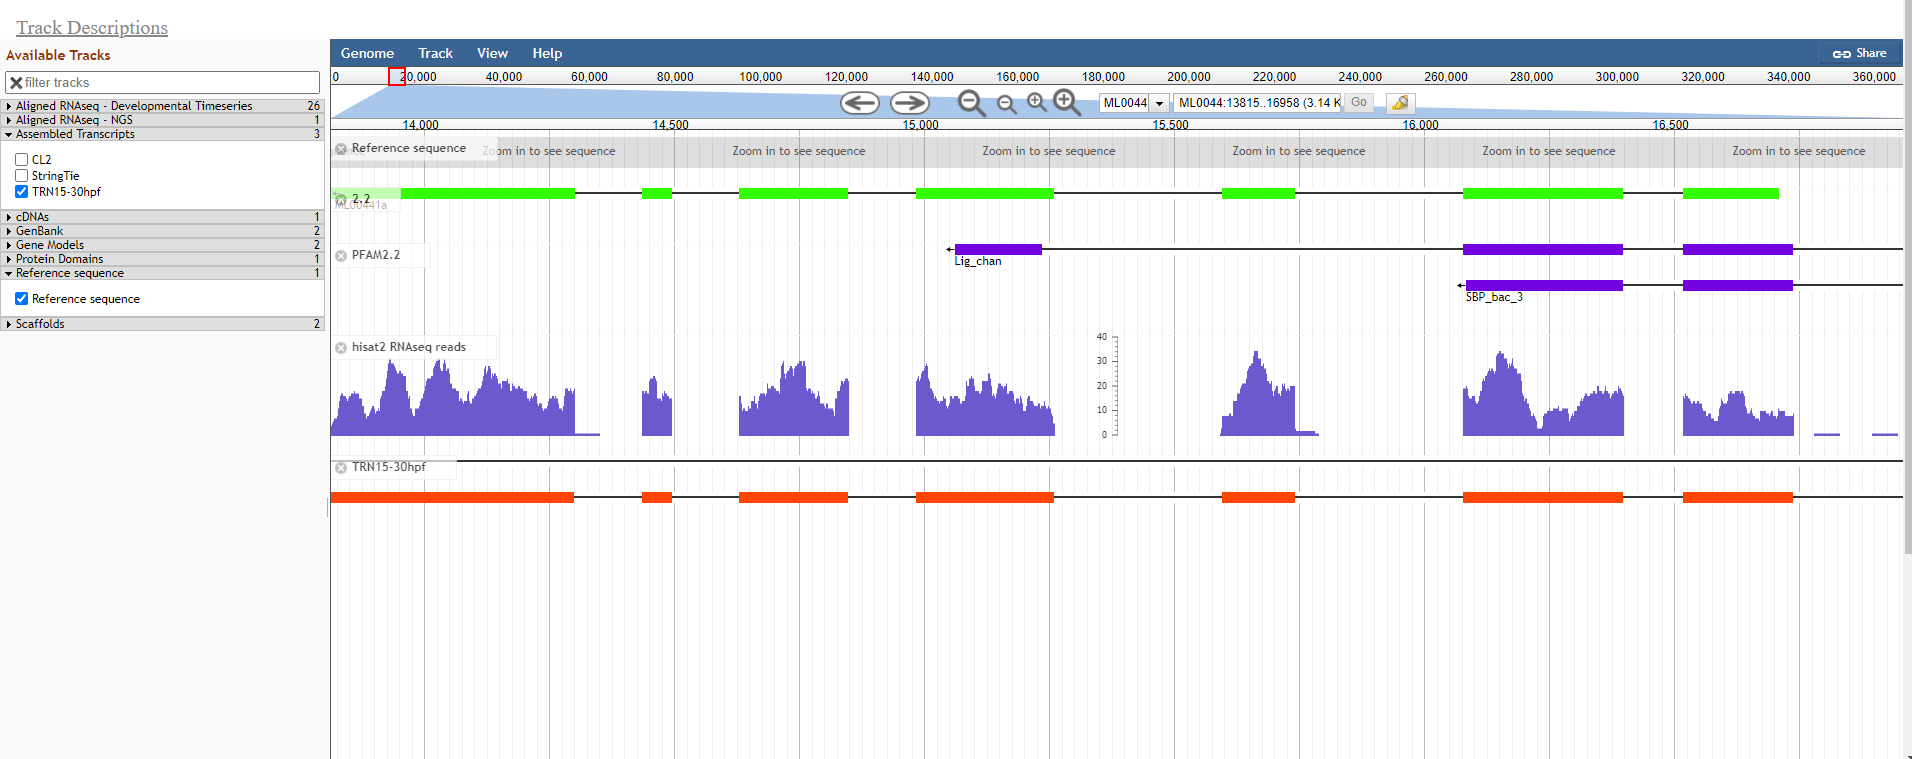
\includegraphics{https://github.com/cbarcl01/CB_BMEG591E-repository/blob/master/Group_Project/Track.png}
\caption{Mnemiopsis leidyi Genome Portal Track for ML00441a}
\end{figure}

This region of interest can be further zoomed in, in order to see the
more information from the Reference sequence as well:

\begin{figure}
\centering
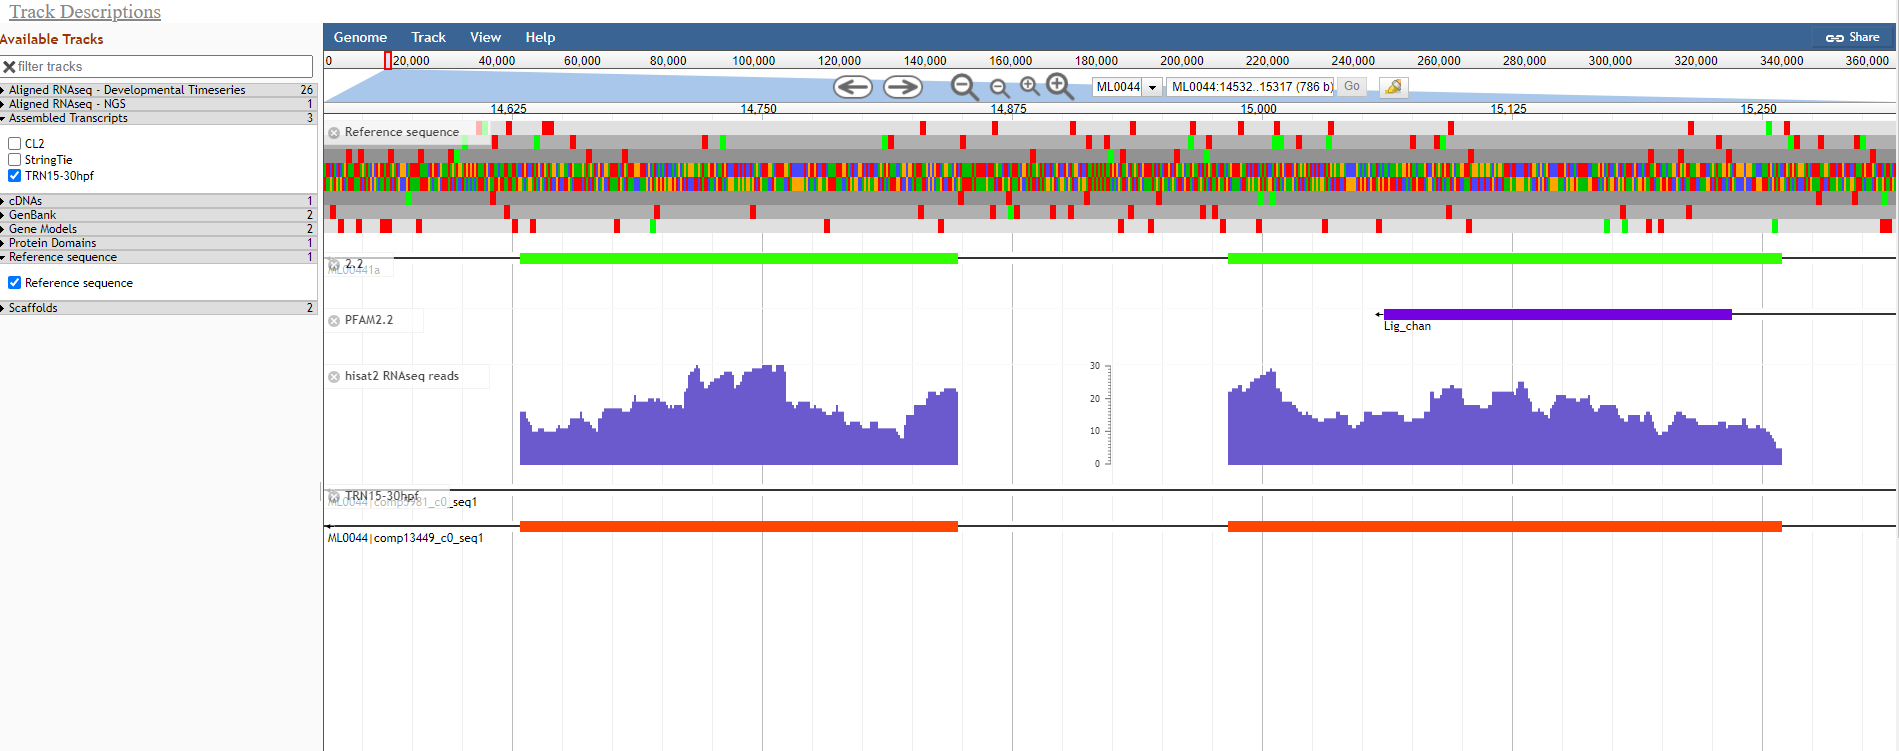
\includegraphics{https://github.com/cbarcl01/CB_BMEG591E-repository/blob/master/Group_Project/Track_Zoom.png}
\caption{Mnemiopsis leidyi Genome Portal Track for ML00441a}
\end{figure}

\hypertarget{blast}{%
\paragraph{2.4.2 BLAST}\label{blast}}

We extracted the nucleotide sequence, as well as the protein sequence
for the target gene region ML00441, as identified in the supplementary
material as a ionotropic glutamate receptor region. Using
\href{https://blast.ncbi.nlm.nih.gov/Blast.cgi}{NCBI BLAST}, we blasted
the first the nucleotide, followed by the protein sequence to identify
similar sequences. The top results were ionotropic glutamate receptors
for other ctenophore species.

BLAST describe the E value (the expect value) as the random chance we
could ``expect'' to get a hit when searching the database of a
particular size, in other words the E value describes the random
background noise. The lower the E-value (the closer it is to zero), the
more ``significant'' the match
is\href{https://blast.ncbi.nlm.nih.gov/Blast.cgi?CMD=Web\&PAGE_TYPE=BlastDocs\&DOC_TYPE=FAQ\#:~:text=The\%20Expect\%20value\%20(E)\%20is,describes\%20the\%20random\%20background\%20noise}{REF}.
The results can be seen below:

\textbf{Nucleotide Blast search results}

\begin{figure}
\centering
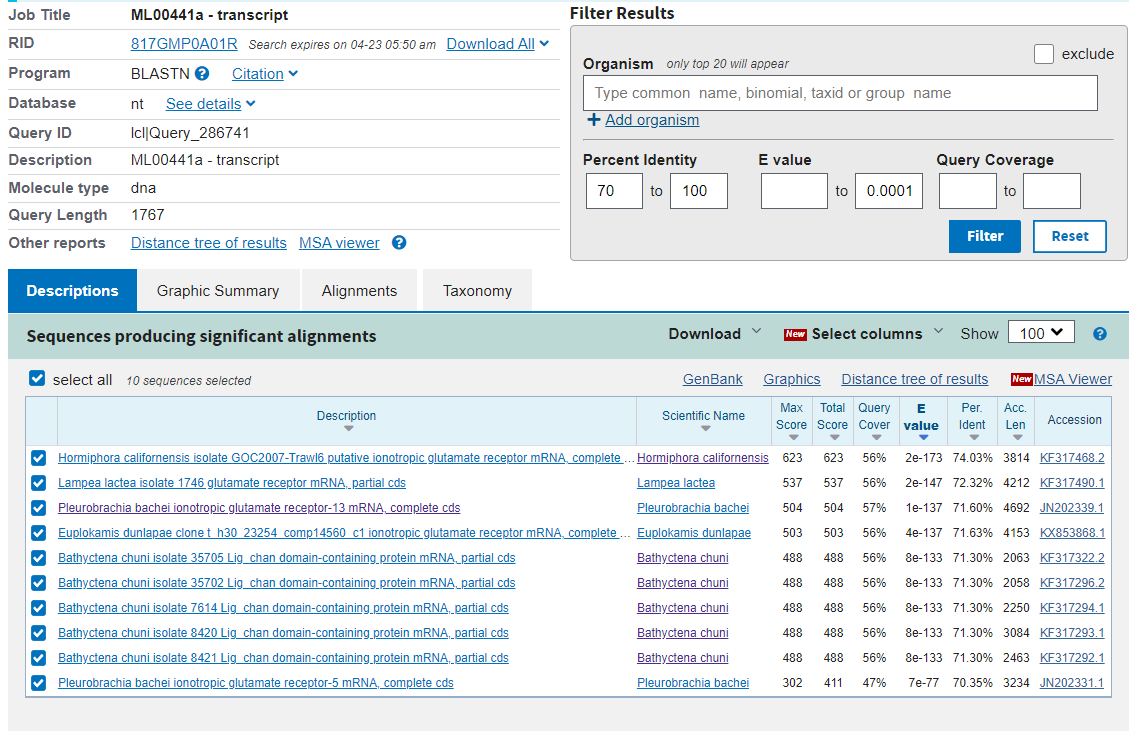
\includegraphics{https://github.com/cbarcl01/CB_BMEG591E-repository/blob/master/Group_Project/BLASTN_ML00441a.png}
\caption{Nucleotide Blast Search results}
\end{figure}

\textbf{Nucleotide Blast search results}

\begin{figure}
\centering
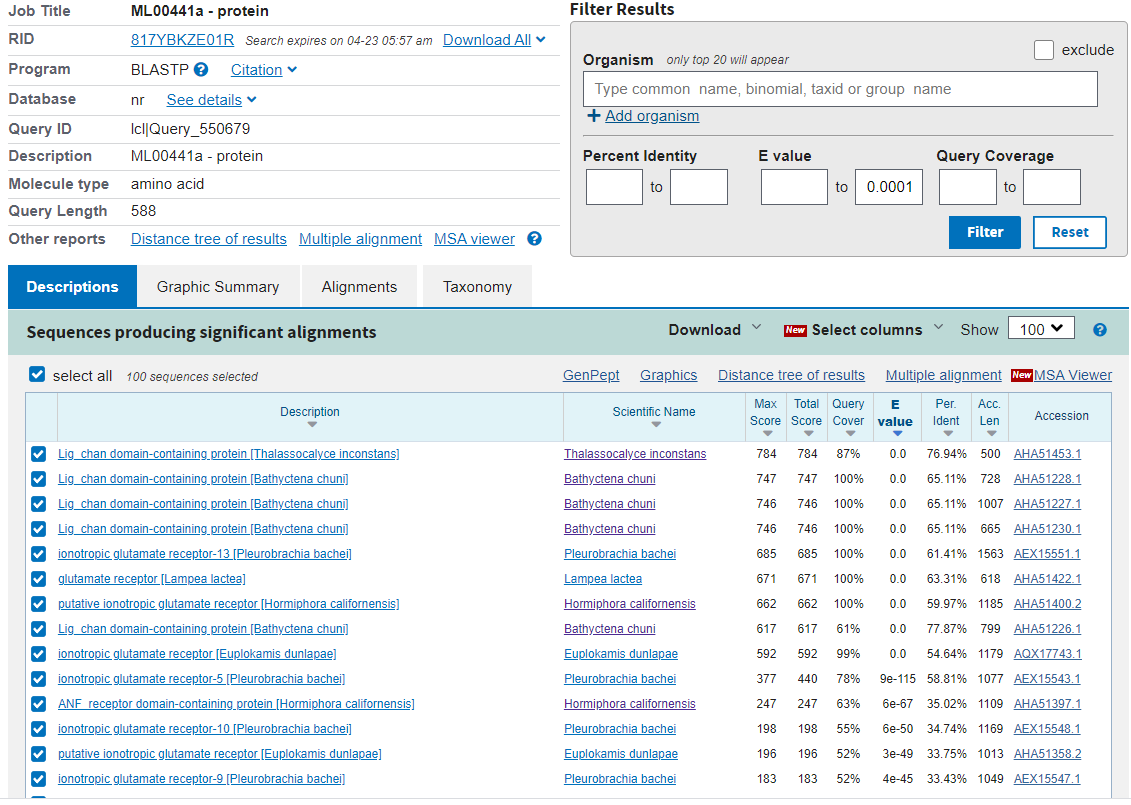
\includegraphics{https://github.com/cbarcl01/CB_BMEG591E-repository/blob/master/Group_Project/BLASTP_ML00441a.png}
\caption{Protein Blast Search results}
\end{figure}

\hypertarget{create-a-phylogenetic-tree-using-figtree.}{%
\paragraph{2.4.3 Create a Phylogenetic Tree using
FigTree.}\label{create-a-phylogenetic-tree-using-figtree.}}

Firstly we downloaded the .fasta protein sequences identified above into
a single file. Then we retrieved published sequences from GenBank for a
number of AMPA (GRIA) and delta2-like (GRID) glutamate receptors, as
described in the original study. Human protein sequences (GRID1
(Accession AAH39263.1), GRID2 (Accession AAH99654.1), GRIA1 (Accession
XP\_016864881.1), GRIA2(Accession AAH10574.1)) and cnidaria sequences
for glutamate receptorionotropic, kainate 2-like (Accession
XP\_029213800.1, XP\_027046759.1 and XP\_022792571.1) were also added to
.fasta file along with the sequence for ML00441a, in a slight
modification to the supplementary material.

\begin{longtable}[]{@{}llll@{}}
\toprule
\begin{minipage}[b]{(\columnwidth - 3\tabcolsep) * \real{0.25}}\raggedright
Description\strut
\end{minipage} &
\begin{minipage}[b]{(\columnwidth - 3\tabcolsep) * \real{0.35}}\raggedright
Scientific Name\strut
\end{minipage} &
\begin{minipage}[b]{(\columnwidth - 3\tabcolsep) * \real{0.14}}\raggedright
Group\strut
\end{minipage} &
\begin{minipage}[b]{(\columnwidth - 3\tabcolsep) * \real{0.25}}\raggedright
Accession\strut
\end{minipage}\tabularnewline
\midrule
\endhead
\begin{minipage}[t]{(\columnwidth - 3\tabcolsep) * \real{0.25}}\raggedright
Lig\_chan domain-containing protein\strut
\end{minipage} &
\begin{minipage}[t]{(\columnwidth - 3\tabcolsep) * \real{0.35}}\raggedright
Thalassocalyce inconstans\strut
\end{minipage} &
\begin{minipage}[t]{(\columnwidth - 3\tabcolsep) * \real{0.14}}\raggedright
Ctenophora\strut
\end{minipage} &
\begin{minipage}[t]{(\columnwidth - 3\tabcolsep) * \real{0.25}}\raggedright
AHA51453.1\strut
\end{minipage}\tabularnewline
\begin{minipage}[t]{(\columnwidth - 3\tabcolsep) * \real{0.25}}\raggedright
Lig\_chan domain-containing protein\strut
\end{minipage} &
\begin{minipage}[t]{(\columnwidth - 3\tabcolsep) * \real{0.35}}\raggedright
Bathyctena chuni\strut
\end{minipage} &
\begin{minipage}[t]{(\columnwidth - 3\tabcolsep) * \real{0.14}}\raggedright
Ctenophora\strut
\end{minipage} &
\begin{minipage}[t]{(\columnwidth - 3\tabcolsep) * \real{0.25}}\raggedright
AHA51228.1\strut
\end{minipage}\tabularnewline
\begin{minipage}[t]{(\columnwidth - 3\tabcolsep) * \real{0.25}}\raggedright
Lig\_chan domain-containing protein\strut
\end{minipage} &
\begin{minipage}[t]{(\columnwidth - 3\tabcolsep) * \real{0.35}}\raggedright
Bathyctena chuni\strut
\end{minipage} &
\begin{minipage}[t]{(\columnwidth - 3\tabcolsep) * \real{0.14}}\raggedright
Ctenophora\strut
\end{minipage} &
\begin{minipage}[t]{(\columnwidth - 3\tabcolsep) * \real{0.25}}\raggedright
AHA51227.1\strut
\end{minipage}\tabularnewline
\begin{minipage}[t]{(\columnwidth - 3\tabcolsep) * \real{0.25}}\raggedright
Lig\_chan domain-containing protein\strut
\end{minipage} &
\begin{minipage}[t]{(\columnwidth - 3\tabcolsep) * \real{0.35}}\raggedright
Bathyctena chuni\strut
\end{minipage} &
\begin{minipage}[t]{(\columnwidth - 3\tabcolsep) * \real{0.14}}\raggedright
Ctenophora\strut
\end{minipage} &
\begin{minipage}[t]{(\columnwidth - 3\tabcolsep) * \real{0.25}}\raggedright
AHA51230.1\strut
\end{minipage}\tabularnewline
\begin{minipage}[t]{(\columnwidth - 3\tabcolsep) * \real{0.25}}\raggedright
ionotropic glutamate receptor-13\strut
\end{minipage} &
\begin{minipage}[t]{(\columnwidth - 3\tabcolsep) * \real{0.35}}\raggedright
Pleurobrachia bachei\strut
\end{minipage} &
\begin{minipage}[t]{(\columnwidth - 3\tabcolsep) * \real{0.14}}\raggedright
Ctenophora\strut
\end{minipage} &
\begin{minipage}[t]{(\columnwidth - 3\tabcolsep) * \real{0.25}}\raggedright
AEX15551.1\strut
\end{minipage}\tabularnewline
\begin{minipage}[t]{(\columnwidth - 3\tabcolsep) * \real{0.25}}\raggedright
glutamate receptor\strut
\end{minipage} &
\begin{minipage}[t]{(\columnwidth - 3\tabcolsep) * \real{0.35}}\raggedright
Lampea lactea\strut
\end{minipage} &
\begin{minipage}[t]{(\columnwidth - 3\tabcolsep) * \real{0.14}}\raggedright
Ctenophora\strut
\end{minipage} &
\begin{minipage}[t]{(\columnwidth - 3\tabcolsep) * \real{0.25}}\raggedright
AHA51422.1\strut
\end{minipage}\tabularnewline
\begin{minipage}[t]{(\columnwidth - 3\tabcolsep) * \real{0.25}}\raggedright
putative ionotropic glutamate receptor\strut
\end{minipage} &
\begin{minipage}[t]{(\columnwidth - 3\tabcolsep) * \real{0.35}}\raggedright
Hormiphora californensis\strut
\end{minipage} &
\begin{minipage}[t]{(\columnwidth - 3\tabcolsep) * \real{0.14}}\raggedright
Ctenophora\strut
\end{minipage} &
\begin{minipage}[t]{(\columnwidth - 3\tabcolsep) * \real{0.25}}\raggedright
AHA51400.2\strut
\end{minipage}\tabularnewline
\begin{minipage}[t]{(\columnwidth - 3\tabcolsep) * \real{0.25}}\raggedright
Lig\_chan domain-containing protein\strut
\end{minipage} &
\begin{minipage}[t]{(\columnwidth - 3\tabcolsep) * \real{0.35}}\raggedright
Bathyctena chuni\strut
\end{minipage} &
\begin{minipage}[t]{(\columnwidth - 3\tabcolsep) * \real{0.14}}\raggedright
Ctenophora\strut
\end{minipage} &
\begin{minipage}[t]{(\columnwidth - 3\tabcolsep) * \real{0.25}}\raggedright
AHA51226.1\strut
\end{minipage}\tabularnewline
\begin{minipage}[t]{(\columnwidth - 3\tabcolsep) * \real{0.25}}\raggedright
ionotropic glutamate receptor\strut
\end{minipage} &
\begin{minipage}[t]{(\columnwidth - 3\tabcolsep) * \real{0.35}}\raggedright
Euplokamis dunlapae\strut
\end{minipage} &
\begin{minipage}[t]{(\columnwidth - 3\tabcolsep) * \real{0.14}}\raggedright
Ctenophora\strut
\end{minipage} &
\begin{minipage}[t]{(\columnwidth - 3\tabcolsep) * \real{0.25}}\raggedright
AQX17743.1\strut
\end{minipage}\tabularnewline
\begin{minipage}[t]{(\columnwidth - 3\tabcolsep) * \real{0.25}}\raggedright
ionotropic glutamate receptor-5\strut
\end{minipage} &
\begin{minipage}[t]{(\columnwidth - 3\tabcolsep) * \real{0.35}}\raggedright
Pleurobrachia bachei\strut
\end{minipage} &
\begin{minipage}[t]{(\columnwidth - 3\tabcolsep) * \real{0.14}}\raggedright
Ctenophora\strut
\end{minipage} &
\begin{minipage}[t]{(\columnwidth - 3\tabcolsep) * \real{0.25}}\raggedright
AEX15543.1\strut
\end{minipage}\tabularnewline
\begin{minipage}[t]{(\columnwidth - 3\tabcolsep) * \real{0.25}}\raggedright
GRID1 protein\strut
\end{minipage} &
\begin{minipage}[t]{(\columnwidth - 3\tabcolsep) * \real{0.35}}\raggedright
Homo sapiens Mammalia\strut
\end{minipage} &
\begin{minipage}[t]{(\columnwidth - 3\tabcolsep) * \real{0.14}}\raggedright
AAH39263.1\strut
\end{minipage} &
\begin{minipage}[t]{(\columnwidth - 3\tabcolsep) * \real{0.25}}\raggedright
\strut
\end{minipage}\tabularnewline
\begin{minipage}[t]{(\columnwidth - 3\tabcolsep) * \real{0.25}}\raggedright
GRID2 protein\strut
\end{minipage} &
\begin{minipage}[t]{(\columnwidth - 3\tabcolsep) * \real{0.35}}\raggedright
Homo sapiens Mammalia\strut
\end{minipage} &
\begin{minipage}[t]{(\columnwidth - 3\tabcolsep) * \real{0.14}}\raggedright
AAH99654.1\strut
\end{minipage} &
\begin{minipage}[t]{(\columnwidth - 3\tabcolsep) * \real{0.25}}\raggedright
\strut
\end{minipage}\tabularnewline
\begin{minipage}[t]{(\columnwidth - 3\tabcolsep) * \real{0.25}}\raggedright
GRIA1 glutamate receptor 1 isoform X1\strut
\end{minipage} &
\begin{minipage}[t]{(\columnwidth - 3\tabcolsep) * \real{0.35}}\raggedright
Homo sapiens Mammalia\strut
\end{minipage} &
\begin{minipage}[t]{(\columnwidth - 3\tabcolsep) * \real{0.14}}\raggedright
XP\_016864881.1\strut
\end{minipage} &
\begin{minipage}[t]{(\columnwidth - 3\tabcolsep) * \real{0.25}}\raggedright
\strut
\end{minipage}\tabularnewline
\begin{minipage}[t]{(\columnwidth - 3\tabcolsep) * \real{0.25}}\raggedright
GRIA2 protein\strut
\end{minipage} &
\begin{minipage}[t]{(\columnwidth - 3\tabcolsep) * \real{0.35}}\raggedright
Homo sapiens Mammalia\strut
\end{minipage} &
\begin{minipage}[t]{(\columnwidth - 3\tabcolsep) * \real{0.14}}\raggedright
AAH10574.1\strut
\end{minipage} &
\begin{minipage}[t]{(\columnwidth - 3\tabcolsep) * \real{0.25}}\raggedright
\strut
\end{minipage}\tabularnewline
\begin{minipage}[t]{(\columnwidth - 3\tabcolsep) * \real{0.25}}\raggedright
glutamate receptor ionotropic, kainate 2-like\strut
\end{minipage} &
\begin{minipage}[t]{(\columnwidth - 3\tabcolsep) * \real{0.35}}\raggedright
Acropora millepora Cnidaria\strut
\end{minipage} &
\begin{minipage}[t]{(\columnwidth - 3\tabcolsep) * \real{0.14}}\raggedright
XP\_029213800.1\strut
\end{minipage} &
\begin{minipage}[t]{(\columnwidth - 3\tabcolsep) * \real{0.25}}\raggedright
\strut
\end{minipage}\tabularnewline
\begin{minipage}[t]{(\columnwidth - 3\tabcolsep) * \real{0.25}}\raggedright
glutamate receptor ionotropic, kainate 2-like\strut
\end{minipage} &
\begin{minipage}[t]{(\columnwidth - 3\tabcolsep) * \real{0.35}}\raggedright
Pocillopora damicornis Cnidaria\strut
\end{minipage} &
\begin{minipage}[t]{(\columnwidth - 3\tabcolsep) * \real{0.14}}\raggedright
XP\_027046759.1\strut
\end{minipage} &
\begin{minipage}[t]{(\columnwidth - 3\tabcolsep) * \real{0.25}}\raggedright
\strut
\end{minipage}\tabularnewline
\begin{minipage}[t]{(\columnwidth - 3\tabcolsep) * \real{0.25}}\raggedright
glutamate receptor ionotropic, kainate 2-like\strut
\end{minipage} &
\begin{minipage}[t]{(\columnwidth - 3\tabcolsep) * \real{0.35}}\raggedright
Stylophora pistillata Cnidaria\strut
\end{minipage} &
\begin{minipage}[t]{(\columnwidth - 3\tabcolsep) * \real{0.14}}\raggedright
XP\_022792571.1\strut
\end{minipage} &
\begin{minipage}[t]{(\columnwidth - 3\tabcolsep) * \real{0.25}}\raggedright
\strut
\end{minipage}\tabularnewline
\bottomrule
\end{longtable}

Secondly, we generated a multiple sequence alignment using the EBI tool
\textbf{MU}ltiple \textbf{S}equence \textbf{C}omparison by \textbf{L}og
- \textbf{E}xpectation, known as
\href{https://www.ebi.ac.uk/Tools/msa/muscle/}{MUSCLE}, with the output
defined as Pearson/FASTA {[}28{]}.

\begin{Shaded}
\begin{Highlighting}[]
\ExtensionTok{conda}\NormalTok{ install {-}c bioconda muscle}
\ExtensionTok{muscle}\NormalTok{ {-}in ./BLAST\_P.fasta {-}quiet {-}fasta {-}out BLASTP\_Aligned.fasta}
\end{Highlighting}
\end{Shaded}

Finally we ran a Neighbor Joining analysis using the EBI phylogeny tool
\href{https://www.ebi.ac.uk/Tools/phylogeny/simple_phylogeny/}{Simple
Phylogeny}, which was used as the input to the FigTree software to
generate the tree. FigTree was used to colour annotate the tree, with
Biorender utilised to add some additional annotation. FigTree is
available for download
\href{http://tree.bio.ed.ac.uk/software/figtree/}{here}.

\begin{Shaded}
\begin{Highlighting}[]
\ExtensionTok{conda}\NormalTok{ install {-}c bioconda muscle}
\ExtensionTok{muscle}\NormalTok{ {-}in ./BLAST\_P.fasta {-}quiet {-}fasta {-}out BLASTP\_Aligned.fasta}
\ExtensionTok{/nfs/public/ro/es/appbin/linux{-}x86\_64/clustalw{-}2.1/bin/clustalw2}\NormalTok{ {-}infile=simple\_phylogeny{-}I20210422{-}022731{-}0145{-}87347698{-}p1m.upfile {-}tree {-}outputtree=phylip {-}clustering=Neighbour{-}joining}
\end{Highlighting}
\end{Shaded}

\begin{figure}
\centering
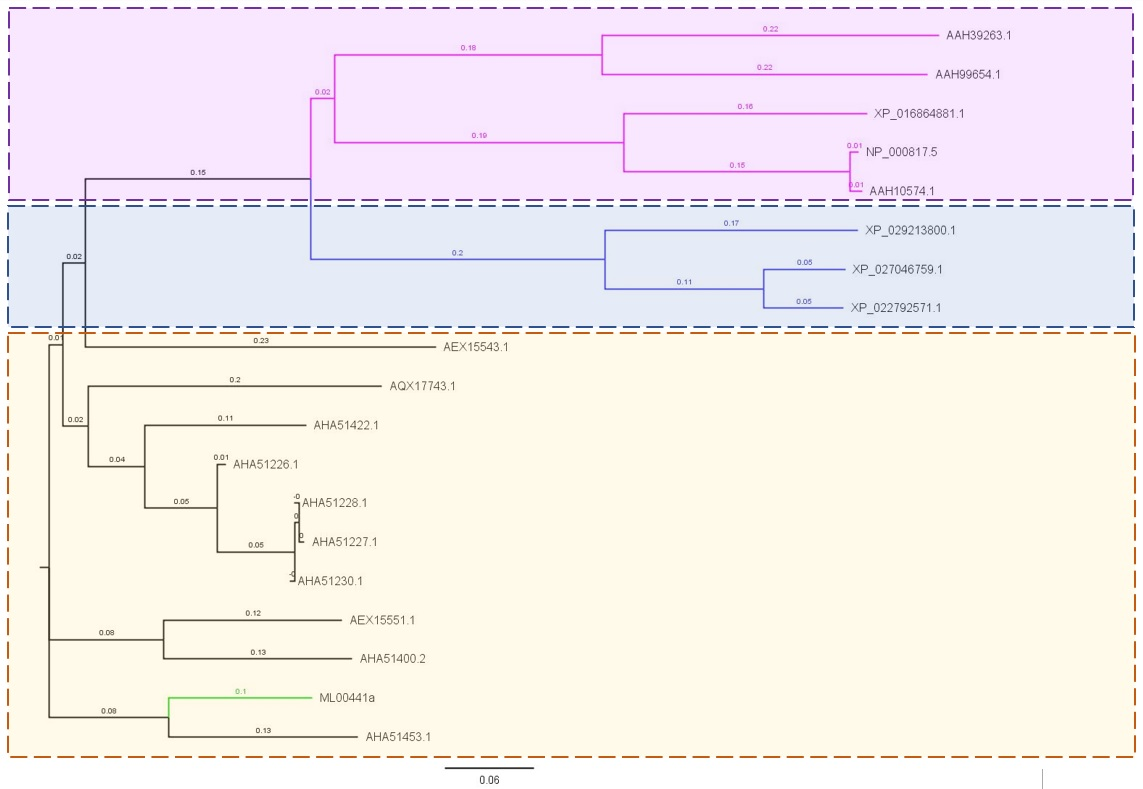
\includegraphics{BLAST_PTree1.jpg}
\caption{Phylogenetic Tree}
\end{figure}

In our tree we can see the Ctenophora as the earliest clade (the
ML00441a gene region is annotated green), with the Cnidaria in a sister
clade (branches annotated blue) to the human gene regions (branches
annotated pink). Interestingly there is a lot of variation within the
Ctenophora, with the ML00441a gene region sitting in a clade distinct
from the other ctenophore species, with \emph{Thalassocalyce
inconstans}.

\hypertarget{discussion}{%
\subsection{3. Discussion}\label{discussion}}

Here, we attempted to familiarize with most of the fundamental steps of
the \emph{M. leidyi} sequencing project. The gap between sample
collections and publishing of the Genome Portal/Science paper indicates
that it took a minimum of two years to successfully assemble and
annotate the genome of this relatively unknown early metazoan. Our
attempts to replicate the BLAT alignment were partially successful,
where we reported that 99.4\% and 98.8\% of the ESTs and transcripts
respectively were mapped with BLAT. Indeed, the authors provided the
scores of 99.4\% and 99.2\% (we consider this margin to be negligible)
for the same statistic. Due to issues while running baa.pl/Isoblat, the
other two meaningful statistics were not generated on our end. We
speculate that this is due to incompatibilities of the tool with its
dependencies - Isoblat was last updated three years ago. Nowadays, tools
like GenomeQC {[}29{]} are often used for assessment of assembly
quality.

We attempted to replicate the alignment using Bowtie2. Surprisingly,
Bowtie2 alignment scores fell under 60\% (55.63\% and 53.37\% for ESTs
and transcripts alignment to the genome respectively). We attempted to
assess the reasons that might explain the differences. BLAT is a tool
that operates pretty much like BLAST {[}30{]}, but there are a few
differences in its structure. While BLAST targets GenBank sequences,
BLAT indexes the target genome, similarly to Bowtie2. BLAT indexing
approach is known as hash-based - a data structure format that associate
strings to a hash value through hash functions, resulting in a hash
table {[}31{]}, and the tool builds this index by finding all the
non-overlapping 11-mers not heavily involved in repeats {[}15{]}.
Bowtie2, on the other hand, uses an FM-index based on a Burrows-Wheeler
Approach {[}27{]} through an algorithm known as Blockwise {[}32{]}.

In spite of indexing being a compression step to speed up alignment, it
is known that different compression algorithms and different data
structure approaches can yield slight differences in output however, we
are not confident this can explain the large discrepancy seen in this
analysis. In addition, BLAT applies a gap-aware approach, whereas
Bowtie2 does not. Blat also recognizes and work around introns and
exons, being generally designed to work better with the alignment of
ESTs to an assembled genome. The result of this comparison highlights
the importance of choosing the appropriate alignment software for the
research project. For this specific dataset, it is unlikely that Bowtie2
is able to yield meaningful results, whereas BLAT was able to.
Furthermore, with the development of HiFi reads, a highly accurate long
read generated from circular consensus sequencing (99\% accuracy), a
useful future study would be to repeat the sequence study using HiFi
reads. In this case a long read assembler such as minimap2 or Pbmm2 may
be preferential.

We report genomic GC content at around 37\% in all our measurement
approaches. The authors report 38.86\%. We assume the 1\% discrepancy
comes from the extra steps the authors employed to mask repeats detected
using RepeatMasker {[}33{]}, and conclude that we achieve a satisfactory
match, given this condition.

Our genome annotation attempt using Augustus missed a few data
processing steps they authors initially made, including masking repeats
and incorporating additional 161 cDNA sequences. The authors reported
29,359 predicted protein-coding loci. In comparison to HMMGene (that
predicted 13,948 genes), it predicted 15,411 additional loci. Augustus
consistently predicted a higher number of loci than every other employed
tool. By the end, the authors opted for keeping FGENESH and PASA
predictions, evaluated through EVM (EvidenceModeler) {[}25{]}, obtaining
16,845 genes, closer to the reported final number of 16,548 genes after
manual curation of additional sequences.

Nevertheless, Augustus initial value predicted 33,354 genes, predicting
aprox. 4,000 genes more than the expected. Intriguingly, when mapping
the sequences back to the assembled genome using BED-tools, we obtain
29,875 genes, a value much closer to the reported value of the original
study. As described, this increment is likely caused by the missing
steps (and for the final value, likely cause by the missing 161 CDNA
sequences incorporated on the hints file). Unsurprisingly, running our
Augustus prediction sequences against the reference genome via BLASTp
reveals that the predicted genes match consistently known annotated
\emph{M. leidyi} genes (we were able to consistently find sequences
scoring high identity and significant e-value).

Regarding phylogeny, the original study utilised maximum-likelihood
analysis methods, in addition to Bayesian analysis (using PhyloBayes),
of two datasets; a whole genome dataset comprised of 13 animals and a an
EST set of 58 animals. As mentioned at the beginning of this assignment,
on average the runs took 205 days to complete and were out of scope for
this project. Instead we attempted to replicate the ionotropic glutamate
receptor phylogeny of human and ctenophore as described in the
supplementary material.

We utilised the MUSCLE and Simple Phylogeny tools of EBI to do this and
found results which supported that of the initial study. The tree
demonstrates that the ionotropic glutamate receptors of ctenophores are
not direct orthologs to AMPA (GRIA), or delta2-like (GRID) glutamate
receptors of humans, however they support the theory that ctenophore
receptors form a sister clade to the bilaterian glutamte receptors
{[}10{]}, as can be seen from the distinction between the Ctenophore and
human cladesin our phylogenetic tree. As an addition to the the study we
also included relevant sequences from Cnidaria species, which was also
clearly in a distinct clade. Our tree shows Ctenophora at the base of
metazoa, with Cnidaria sister to Bilateria (human), which confirms
results seen by later studies {[}ref 6{]}. Interestingly, we can see a
variety of gene content within the ctenophora as demonstrated by the
phylogenetic tree, which may be worth further investigation in future
studies.

Extensive BLAST searches and querying of GenBank did not provide
orthologs of these receptors in the sponge \emph{Amphipedon
queenslandica}, however this have been identified in eight other sponges
{[}10{]}. Further investigation of these orthologs and their
phylogenetic placement compared to the sequences in our tree and that of
the original study, could be useful in providing insights to the
phylogenetic placement of these non-bilaterian groups - particularly
given the lack of a complex nerve system in sponges {[}5-6, 10{]}

\hypertarget{conclusion}{%
\subsection{4. Conclusion}\label{conclusion}}

Here, we attempted to partially cover a 2-year long \emph{M. leidyi}
genome sequencing project. We were able to cover essentially 1/3 of the
overall steps, obtaining values that were consistent with the reported
by the authors of the original paper. We faced a number of technical
problems and troubleshooting them forced us to change our planned
structure several times. When we attempted to add novel approaches to a
few of the steps, we realized that it would simply fall away from the
original goal of the project. With that being said, it is clear that
several advances in data transparency were made since 2011 and, although
this particular paper presents most of its data and processes in a
transparent and replicable way, there were steps that lack of clearer
explanations made them unfeasible (e.g.~running our data through PASA
and masking portions of the genome). Nevertheless, we have shown several
steps in a replicable way. More complex annotation, phylogeny analysis,
and manual processes inbetween each major step were unreasonable for our
time-scale. On a biological perspective, this reference genome surely
can be improved with the application of novel approaches such as
long-reads PacBio/Oxford Nanopore platforms. \emph{M. leidyi} remains an
interesting model organism for evolutionary and developmental studies at
the earliest branching Metazoan groups, and said studies surely would
benefit of having a wider community working on improving its reference
genome.

\hypertarget{bibliography}{%
\subsection{5. Bibliography}\label{bibliography}}

\begin{enumerate}
\def\labelenumi{\arabic{enumi}.}
\tightlist
\item
  Van Gestel J, Tarnita CE. On the origin of biological construction,
  with a focus on multicellularity. Proc Natl Acad Sci U S A.
  2017;114(42):11018-11026. \url{doi:10.1073/pnas.1704631114}
  \textless\textless\textless\textless\textless\textless\textless{} HEAD
\item
  Bonnert JT. The Origins of Multicellularity. 1998.
\item
  Parfrey LW, Lahr DJG. Building a Multicellular Organism. 2001.
\item
  Ruiz-Trillo I et al.~The origins of multicellularity: a multi-taxon
  genome initiative. Trends Genet. 2007; 23(3):113-118.
\item
  Niklas KJ, Newman SA. The many roads to and from multicellularity. J
  Exp Bot. 2020;71(11):3247-3253. \url{doi:10.1093/jxb/erz547}
\item
  Niklas KJ, Newman SA. The origins of multicellular organisms.
  Published online 2013. \url{doi:10.1111/ede.12013}
\item
  Morris SC. The fossil record and the early evolution of the Metazoa.
  1993.
\item
  Sebé-Pedrós A, Degnan BM, Ruiz-Trillo I. The origin of Metazoa: A
  unicellular perspective. Nature Reviews Genetics. 2017;18(8):498-512.
\item
  Moreland RT, Nguyen AD, Ryan JF, Baxevanis AD. The Mnemiopsis Genome
  Project Portal: Integrating new gene expression resources and
  improving data visualization. Database. 2020;2020(1):1-9.
  \url{doi:10.1093/database/baaa029}
\item
  Ryan JF, Pang K, Schnitzler CE, et al.~The genome of the ctenophore
  Mnemiopsis leidyi and its implications for cell type evolution.
  Science (80- ). 2013;342(6164). \url{doi:10.1126/science.1242592}
\item
  Ryan JF, Pang K, Mullikin JC, Martindale MQ, Baxevanis AD. The
  homeodomain complement of the ctenophore Mnemiopsis leidyi suggests
  that Ctenophora and Porifera diverged prior to the ParaHoxozoa.
  Evodevo. 2010;1(1):1-18. \url{doi:10.1186/2041-9139-1-9}
\item
  Ryan JF. Did the ctenophore nervous system evolve independently?
  Zoology. 2014;117(4):225-226. \url{doi:10.1016/j.zool.2014.06.001}
\item
  Moroz LL, Kocot KM, Citarella MR, et al.~The ctenophore genome and the
  evolutionary origins of neural systems. Nature.
  2014;510(7503):109-114. \url{doi:10.1038/nature13400}
\item
  Mullikin JC, Ning Z. The phusion assembler. Genome research. 2003 Jan
  1;13(1):81-90.
\item
  Kent WJ. BLAT---the BLAST-like alignment tool. Genome research. 2002
  Apr 1;12(4):656-64.
\item
  Ryan JF. Baa. pl: a tool to evaluate de novo genome assemblies with
  RNA transcripts. arXiv preprint arXiv:1309.2087. 2013 Sep 9.
\item
  Grabherr MG, Haas BJ, Yassour M, Levin JZ, Thompson DA, Amit I,
  Adiconis X, Fan L, Raychowdhury R, Zeng Q, Chen Z. Trinity:
  reconstructing a full-length transcriptome without a genome from
  RNA-Seq data. Nature biotechnology. 2011 Jul;29(7):644.
\item
  Trapnell C, Pachter L, Salzberg SL. TopHat: discovering splice
  junctions with RNA-Seq. Bioinformatics. 2009 May 1;25(9):1105-11.
\item
  Trapnell C, Roberts A, Goff L, Pertea G, Kim D, Kelley DR, Pimentel H,
  Salzberg SL, Rinn JL, Pachter L. Differential gene and transcript
  expression analysis of RNA-seq experiments with TopHat and Cufflinks.
  Nature protocols. 2012 Mar;7(3):562.
\item
  Haas BJ, Delcher AL, Mount SM, Wortman JR, Smith Jr RK, Hannick LI,
  Maiti R, Ronning CM, Rusch DB, Town CD, Salzberg SL. Improving the
  Arabidopsis genome annotation using maximal transcript alignment
  assemblies. Nucleic acids research. 2003 Oct 1;31(19):5654-66.
\item
  Zhang SL, Li DF, Zhang GS, Wang JW, Na NI. The prediction of rice gene
  by Fgenesh. Agricultural Sciences in China. 2008 Apr 1;7(4):387-94.
\item
  Stanke M, Keller O, Gunduz I, Hayes A, Waack S, Morgenstern B.
  AUGUSTUS: ab initio prediction of alternative transcripts. Nucleic
  acids research. 2006 Jul 1;34(suppl\_2):W435-9.
\item
  Krogh A. Using database matches with HMMGene for automated gene
  detection in Drosophila. Genome research. 2000 Apr 1;10(4):523-8.
\item
  Yeh RF, Lim LP, Burge CB. Computational inference of homologous gene
  structures in the human genome. Genome research. 2001 May
  1;11(5):803-16.
\item
  Haas BJ, Salzberg SL, Zhu W, Pertea M, Allen JE, Orvis J, White O,
  Buell CR, Wortman JR. Automated eukaryotic gene structure annotation
  using EVidenceModeler and the Program to Assemble Spliced Alignments.
  Genome biology. 2008 Sep;9(1):1-22.
\item
  Moreland RT, Nguyen AD, Ryan JF, Baxevanis AD. The Mnemiopsis Genome
  Project Portal: integrating new gene expression resources and
  improving data visualization. Database. 2020 Jan 1;2020.
\item
  Langdon WB. Performance of genetic programming optimised Bowtie2 on
  genome comparison and analytic testing (GCAT) benchmarks. BioData
  mining. 2015 Jun;8(1):1-7.
\item
  Edgar RC. MUSCLE: a multiple sequence alignment method with reduced
  time and space complexity. BMC bioinformatics. 2004 Dec;5(1):1-9.
\item
  Manchanda N, Portwood JL, Woodhouse MR, Seetharam AS, Lawrence-Dill
  CJ, Andorf CM, Hufford MB. GenomeQC: a quality assessment tool for
  genome assemblies and gene structure annotations. BMC genomics. 2020
  Dec;21(1):1-9.
\item
  Madden T. The BLAST sequence analysis tool. InThe NCBI Handbook
  {[}Internet{]}. 2nd edition 2013 Mar 15. National Center for
  Biotechnology Information (US).
\item
  Stein B, Potthast M. Applying hash-based indexing in text-based
  information retrieval. InProceedings of the 7th Dutch-Belgian
  Information Retrieval Workshop (DIR 07) 2007 Mar 28 (pp.~29-35).
\item
  Kärkkäinen J. Fast BWT in small space by blockwise suffix sorting.
  Theoretical Computer Science. 2007 Nov 22;387(3):249-57.
\item
  Chen N. Using Repeat Masker to identify repetitive elements in genomic
  sequences. Current protocols in bioinformatics. 2004 Mar;5(1):4-10.
\end{enumerate}

\end{document}
